% Präambel
\documentclass[%
12pt,							% Schriftgröße
a4paper,						% Papierformat
oneside, 						% einseitiges (oneside) oder zweiseitiges (twoside) Dokument
listof=totoc, 					% Tabellen- und Abbildungsverzeichnis ins Inhaltsverzeichnis
bibliography=totoc,				% Literaturverzeichnis ins Inhaltsverzeichnis aufnehmen
titlepage, 						% Titlepage-Umgebung statt \maketitle
headsepline, 					% horizontale Linie unter Kolumnentitel
%abstracton,					% Überschrift beim Abstract einschalten, Abstract muss dazu in {abstract}-Umgebung stehen
DIV=12,							% Satzspiegeleinstellung, 12 ist Standar bei KOMA
%BCOR=6mm,						% Bindekorrektur, die den Seitenspiegel um 6mm nach rechts verschiebt,
cleardoublepage=empty,			% Stil einer leeren eingefügten Seite bei Kapitelwechsel
parskip,							% Absatzabstand bei Absatzwechsel einfügen
ngerman
]{scrbook}			
\usepackage{scrhack}
\usepackage[utf8]{inputenc} 	% ermöglicht die direkte Eingabe von Umlauten
\usepackage[T1]{fontenc} 		% Ausgabe aller zeichen in einer T1-Codierung (wichtig für die Ausgabe von Umlauten!)
\usepackage{babel} 	% deutsche Trennungsregeln und Übersetzung der festcodierten Überschriften
\setlength{\parindent}{0ex} 	% bei neuem Abschnitt nicht einrücken
%------
% Folgende Einstellungen entsprechen den Vorgaben der Leitlinien
\usepackage[onehalfspacing]{setspace}
% Ende Leitlinien
%------
%------
% Folgende Einstellungen sind bei größeren Arbeiten mit viel Text zu empfehlen.
% Hierbei oben DIV=16 einstellen und Zeile \usepackage[onehalfspacing]{setspace} auskommentieren.
%\linespread{1.2}\selectfont     % Zeilenabstand erhöhen - größere Werte als 1.2 nicht verwenden!!
% Ende Einstellung große Arbeiten mit viel Text.
%------

\usepackage{siunitx}			% Vereinfachte Eingabe von Einheiten in Formeln
\sisetup{
	number-unit-product = \;,
	inter-unit-product = \:,
	exponent-product = \cdot,
	output-decimal-marker = {,}
}

\usepackage{graphicx}  			% Einbinden von Grafiken erlauben
\usepackage[format=hang,		% Formatierungen von Unter- / Überschriften
font=normal,
labelfont=bf,
justification=RaggedRight,
singlelinecheck=true,
aboveskip=1mm
]{caption}

\usepackage[backend=biber, %% Hilfsprogramm "biber" beim Compilieren nutzen (statt "biblatex" oder "bibtex")
style=alphabetic, %% Zitierstil (siehe Dokumentation)
natbib=true, %% Bereitstellen von natbib-kompatiblen Zitierkommandos
hyperref=true, %% hyperref-Paket verwenden, um Links zu erstellen
]{biblatex}

\addbibresource{literature/literatur4.bib} %bevcrjk r4 ju%

% Folgende Zeilen sind auszukommentieren, falls runde Klammern und ein vgl. bei Zitaten erscheinen sollen.
%\makeatletter
%\renewcommand{\@cite}[2]{(vgl. {#1\if@tempswa , #2\fi})} 
%\renewcommand{\@biblabel}[1]{(#1)}
%\makeatother

\usepackage{pdfpages}

\usepackage{enumitem}			% Erlaubt Änderung der Nummerierung in der Umgebung enumerate

\usepackage{amsmath}			% Ergänzungen für Formeln
\usepackage{textcomp} 			% zum Einsatz von Eurozeichen u. a. Symbolen
\usepackage{eurosym}			% bessere Darstellung Euro-Symbol mit \euro
\newcommand*\diff{\mathop{}\!\mathrm{d}}	% Differentialzeichen
\newcommand*\Diff[1]{\mathop{}\!\mathrm{d^#1}} % Differentialzeichen höherer Ableitung
\newcommand*\jj{\mathop{}\!\mathrm{j}}	% Komplexe Zahl j

\usepackage[					% Einstellunge Paket hyperref
hyperfootnotes=false,			% im pfd-Output Fußnoten nicht verlinken
hidelinks
]{hyperref}

\usepackage{makeidx}			% Paket zur Erstellung eines Index
\usepackage[intoc]{nomencl} 	% zur Erstellung des Abkürzungsberzeichnisses

\usepackage[					% Einstellungen für Fußnoten
bottom,							% Ausrichtung unten
multiple,						% Trennung durch Seperator bei mehreren Fußnoten
hang,
marginal
]{footmisc}

\usepackage{calc}				% Paket zum Berechnen von Längen z.B. 0.8\linewidth

\usepackage{xcolor} 			% einfache Verwendung von Farben in nahezu allen Farbmodellen

\usepackage{listings}			% Darstellung von Quellcode mit den Umgebungen {lstlisting}, \lstinline und \lstinputlisting
\lstset{literate=				% Damit können Umlaute innerhalb Listings geschrieben werden
	{Ö}{{\"O}}1
	{Ä}{{\"A}}1
	{Ü}{{\"U}}1
	{ß}{{\ss}}1
	{ü}{{\"u}}1
	{ä}{{\"a}}1
	{ö}{{\"o}}1
}
\definecolor{mygreen}{rgb}{0,0.6,0}
\definecolor{mygray}{rgb}{0.5,0.5,0.5}
\definecolor{mymauve}{rgb}{0.58,0,0.82}
\lstset{ %
	backgroundcolor=\color{white},   % choose the background color; you must add \usepackage{color} or \usepackage{xcolor}; should come as last argument
	basicstyle=\footnotesize,        % the size of the fonts that are used for the code
	breakatwhitespace=false,         % sets if automatic breaks should only happen at whitespace
	breaklines=true,                 % sets automatic line breaking
	captionpos=t,                    % sets the caption-position to (b) bottom or (t) top
	commentstyle=\color{mygreen},    % comment style
	deletekeywords={...},            % if you want to delete keywords from the given language
	escapeinside={\%*}{*)},          % if you want to add LaTeX within your code
	escapeinside={(*@}{@*)},
	extendedchars=true,              % lets you use non-ASCII characters; for 8-bits encodings only, does not work with UTF-8
	frame=none,	                   	% "single" adds a frame around the code; "none"
	keepspaces=true,                 % keeps spaces in text, useful for keeping indentation of code (possibly needs columns=flexible)
	keywordstyle=\color{blue},       % keyword style
	language=[LaTeX]TeX,             % the language of the code
	morekeywords={*,nomenclature},   % if you want to add more keywords to the set
	numbers=left,                    % where to put the line-numbers; possible values are (none, left, right)
	numbersep=5pt,                   % how far the line-numbers are from the code
	numberstyle=\tiny\color{mygray}, % the style that is used for the line-numbers
	rulecolor=\color{black},         % if not set, the frame-color may be changed on line-breaks within not-black text (e.g. comments (green here))
	showspaces=false,                % show spaces everywhere adding particular underscores; it overrides 'showstringspaces'
	showstringspaces=false,          % underline spaces within strings only
	showtabs=false,                  % show tabs within strings adding particular underscores
	stepnumber=1,                    % the step between two line-numbers. If it's 1, each line will be numbered
	stringstyle=\color{mymauve},     % string literal style
	tabsize=2,	                   % sets default tabsize to 2 spaces
	title=\lstname                   % show the filename of files included with \lstinputlisting; also try caption instead of title
}

\makeindex						% Indexverzeichnis erstellen
\makenomenclature				% Abkürzungsverzeichnis erstellen

% -----------------------------------------------------------------------------------------------------------------
% Zum Aktualisieren des Abkürzungsverzeichnisses (Nomenklatur) bitte auf der Kommandozeile folgenden Befehl aufrufen :
% makeindex <Dateiname>.nlo -s nomencl.ist -o <Dateiname>.nls
% Oder besser: Kann in TexStudio unter Tools-Benutzer als Shortlink angelegt werden
% Konfiguration unter: Optionen-Erzeugen-Benutzerbefehle: makeindex -s nomencl.ist -t %.nlg -o %.nls %.nlo
% -----------------------------------------------------------------------------------------------------------------

% Hier die persönlichen Daten eingeben:

\newcommand{\titel}{Evaluation von Komponenten eines Fahrzeugprototypen mit digitalen Sonderausstattungen}
\newcommand{\untertitel}{}
\newcommand{\arbeit}{Praxisbericht}
\newcommand{\studiengang}{Elektrotechnik}
\newcommand{\studienrichtung}{Fahrzeugelektronik}
\newcommand{\studienschwerpunkt}{Embedded IT}
\newcommand{\autor}{Alexander Köhn}
\newcommand{\matrikelnr}{216 5691}
\newcommand{\kurs}{TFE20-2}
\newcommand{\firma}{Mercedes Benz AG}
\newcommand{\abgabe}{1. September 2022}
\newcommand{\betreuerdhbw}{Prof. Dr.-Ing. Thomas Kibler}
\newcommand{\betreuerfirma}{M.Sc. Christian Bootz}
\newcommand{\jahr}{2022}			% für Angabe im Copyright-Vermerk der Titelseite

% Folgende Zeilen definieren Abkürzungen, um Befehle schneller eingeben zu können
\newcommand{\ua}{\mbox{u.\,a.\ }}
\newcommand{\zB}{\mbox{z.\,B.\ }}
\newcommand{\bs}{$\backslash$}
\newcommand{\usw}{\mbox{u.\,s.\,w.\ }}

% Folgende Zeilen weden benötigt, um Tikz und PGF-Plot-Grafiken einzubinden
\usepackage{pgfplots}
\usepackage{pgfplotstable}
\pgfplotsset{compat=newest,width=0.6\linewidth}
\usepgfplotslibrary{smithchart}
\usepackage{tikz}						% Tikz sollte nach Listings Pakete geladen werden.
\usepackage{fontawesome}
\usetikzlibrary{arrows}
\usetikzlibrary{positioning}
\usetikzlibrary{decorations}
\usetikzlibrary{decorations.pathreplacing}
\hyphenation{Schrift-ar-ten}
\hyphenation{Kom-pers-sions-fak-tor}


% -------------------------------------------------------------------------------------------
%                     Beginn des Dokumenteninhalts
% -------------------------------------------------------------------------------------------
\begin{document}
\let\texteuro\euro						% Eingabe \texteuro, € oder \euro erzeugt gleiches Ergebnis
\setcounter{secnumdepth}{3}				% Nummerierungstiefe fürs Inhaltsverzeichnis
\setcounter{tocdepth}{3}
\sffamily								% für die Titelei serifenlose Schrift verwenden

% ------------------------------ Titelei -----------------------------------------------------

\thispagestyle{plain}
\hypersetup{pageanchor=false}
\begin{titlepage}
\enlargethispage{4.0cm}
\sffamily 								% Serifenlose Grundschrift für die Titelseite einstellen

\parbox{0.5\linewidth}{
\begin{flushleft}
% Hier ggf. ein Logo der Firma
\end{flushleft}
}
\parbox{0.5\linewidth}{
\begin{flushright}
	
\includegraphics[width=0.4\linewidth]{images/DHBW_d_R_FN_46mm_4c}\\[5ex]
\end{flushright}
}
				

\begin{center}

{\fontsize{20.74pt}{24pt}\selectfont
\textbf{\titel}\\[1.5ex]}
{\fontsize{14pt}{17pt}\selectfont
\textbf{\untertitel}\\[5ex]}
{\fontsize{17pt}{20pt}\selectfont
\textbf{\arbeit}\\[2ex]}
{\fontsize{14pt}{17pt}\selectfont
Studiengang \studiengang\\[2ex]}
{\fontsize{12pt}{14pt}\selectfont
Studienrichtung \studienrichtung\\[1ex]
Duale Hochschule Baden-Württemberg Ravensburg, Campus Friedrichshafen\\[5ex]
von\\[1ex]
\autor\\[15ex]}


\end{center}

\begin{flushleft}
{\fontsize{12pt}{14pt}\selectfont
\begin{tabular}{ll}
Abgabedatum:					& \quad \abgabe \\
Bearbeitungszeitraum:		   		& \quad 04.04.2022 - 31.08.2022   \\ 
Matrikelnummer: 			& \quad \matrikelnr \\ 
Kurs: 							& \quad \kurs \\
Ausbildungsfirma:	 			& \quad \firma \\ 
Betreuer der Ausbildungsfirma:  & \quad \betreuerfirma \\ 
Gutachter der Dualen Hochschule: & \quad \betreuerdhbw \\ [2ex]
\end{tabular}
}
\end{flushleft}
%%%%% Nachfolgende Zeilen einkommentieren, wenn Copyrightvermerk gewünscht ist
%\begin{flushleft}
%{\fontsize{11pt}{13pt}\selectfont
%Copyrightvermerk:\\
%Dieses Werk einschließlich seiner Teile ist \textbf{urheberrechtlich geschützt}. Jede Verwertung außerhalb der engen Grenzen des Urheberrechtgesetzes ist ohne Zustimmung des Autors unzulässig und strafbar. Das gilt insbesondere für Vervielfältigungen, Übersetzungen, Mikroverfilmungen sowie die Einspeicherung und Verarbeitung in elektronischen Systemen.
%}
%\end{flushleft}
%\begin{flushright}
%{\fontsize{11pt}{13pt}\selectfont \copyright{} \jahr }
%\end{flushright}
\end{titlepage}

\cleardoublepage
\hypersetup{pageanchor=true}
 				% erzeugt die Titelseite
\pagenumbering{roman}					% kleine, römische Seitenzahlen für Titelei
%% Ggf. folgende Zeile auskommentieren, falls der Sperrvermerk gewünscht ist.
\chapter*{Sperrvermerk} %*-Variante sorgt dafür, das der Sperrvermerk nicht im Inhaltsverzeichnis auftaucht
gemäß Ziffer 1.1.13 der Anlage 1 zu §§ 3, 4 und 5  der Studien- und Prüfungsordnung für die Bachelorstudiengänge im Studienbereich Technik der Dualen Hochschule Baden-Württemberg vom 29.09.2017 in der Fassung vom 25.07.2018:

Der Inhalt dieser Arbeit darf weder als Ganzes noch in Auszügen Personen außerhalb des Prüfungsprozesses und des Evaluationsverfahrens zugänglich gemacht werden, sofern keine anders lautende Genehmigung vom Dualen Partner vorliegt.\\[6ex]

Stuttgart, den 1. September 2022 \\[1ex]

\rule[-0.2cm]{5cm}{0.5pt} \\

\textsc{\autor} \\[10ex]

\chapter*{Erklärung} %*-Variante sorgt dafür, dass die Erklärung nicht im Inhaltsverzeichnis auftaucht

gemäß Ziffer 1.1.13 der Anlage 1 zu §§ 3, 4 und 5  der Studien- und Prüfungsordnung für die Bachelorstudiengänge im Studienbereich Technik der Dualen Hochschule Baden-Württemberg vom 29.09.2017 in der Fassung vom 25.07.2018.

Ich versichere hiermit, dass ich meine Projektarbeit mit dem Thema:

\begin{quote}
	\textit{\titel} \textit{ \untertitel }
\end{quote}

selbstständig verfasst und keine anderen als die angegebenen Quellen und Hilfsmittel benutzt habe. Ich versichere zudem, dass die eingereichte elektronische Fassung mit der gedruckten Fassung übereinstimmt.\\[6ex]

Stuttgart, den 1. September 2022 \\[1ex]

\rule[-0.2cm]{5cm}{0.5pt} \\

\textsc{\autor} \\[10ex]

\rmfamily

\thispagestyle{empty}

\cleardoublepage

 				% Einbinden der eidestattlichen Erklärung
\chapter*{Kurzfassung} %*-Variante sorgt dafür, das Abstract nicht im Inhaltsverzeichnis auftaucht
Die folgende Arbeit untersucht die Komponenten eines Fahrzeugprototypen anhand von definierten Kriterien. Das Fahrzeug ist für die Erzeugung einer künstlerischen Gesamtinszenierung mit unterschiedlichen Bildschirmen, Videoprojektoren und Lichterzeugern ausgestattet. \\
Die Untersuchungsergebnisse wurden durch eigenständige Recherche und mit Fachleuten für einzelne Gebiete ermittelt. Das Ziel der Untersuchung ist mit den Analyseergebnissen Konzepte für die Ansteuerung der Komponenten an bestehende Fahrzeugarchitekturen zu entwickeln und diese unterschiedlichen Konzepte bewerten. \\
Das Konzept mit einer Anbindung der hoch auflösenden Elemente an Automotive Ethernet oder MOST (Media Oriented Systems Transport) und die Anbindung der weniger Datenintensiven Elemente an den CAN Bus (Controller Area Network) wurde unter den definierten Aspekten als das effektivste bewertet.
\cleardoublepage   			% Einbinden des Abstracts

\tableofcontents						% Erzeugen des Inhalsverzeichnisses
\cleardoublepage

% --------------------------------------------------------------------------------------------
%                    Inhalt der Bachelorarbeit
%---------------------------------------------------------------------------------------------
\pagenumbering{arabic}					% arabische Seitenzahlen für den Hauptteil

\rmfamily

\chapter{Einleitung}
\label{cha:Einleitung}
Das Ziel dieser Arbeit ist basierend auf einer Technischen Bewertung eines Fahrzeugprototypen Möglichkeiten aufzuzeigen wie die dort verwendeten Technologien und Komponenten in Serienfahrzeuge integriert werden können.

Beispiele für verwendete digitalen Technologien in dieser Arbeit sind Non-Fungible Token (NFT\nomenclature{NFT}{Non-Fungible Token}), Virtual Reality (VR\nomenclature{VR}{Virtual Reality}) und Künstliche Intelligenz (KI\nomenclature{KI}{Künstliche Intelligenz}).
Ein bestehender Fahrzeugprototyp mit erweiterten Individualisierungsmöglichkeiten wurde genutzt, um Möglichkeiten für technische Änderungen im Fahrzeug zu zeigen.

Die Arbeit ist wie folgt gegliedert:\\
Zuerst werden in Kapitel \ref{cha:Grundlagen} Grundlagen zu unterschiedlichen für diese Arbeit wichtige Technologien erläutert und der Fahrzeugprototyp in Kapitel \ref{cha:Prototyp} näher beschrieben. In Kapitel \ref{cha:Kriterien} werden Kriterien für den Einzug von Individualisierungsmöglichkeiten durch neuartige Komponenten im Fahrzeug aufgezählt und anschließend in Kapitel \ref{cha:Bewertung} der Prototyp anhand dieser bewertet. Mithilfe der Bewertung bildet Kapitel \ref{cha:Konzeptentwurf} einen möglichen Entwurf für das Einbinden der digitalen Technologien. Auf Basis des Konzeptentwurfs wird in Kapitel \ref{cha:Verifikation} darüber unter unterschiedlichen Gesichtspunkten diskutiert. Abschließend wird in Kapitel \ref{cha:zusammenfassung} die Arbeit auf wesentliche Erläuterungen zusammengefasst.
\chapter{Grundlagen}
\label{cha:Grundlagen}
Im folgenden werden für diese Arbeit notwendige Grundlagen zu unterschiedlichen Technologien und Wissensbereiche erarbeitet. 
Zuerst wird die menschliche Wahrnehmung erläutert, da auf diesen die Kriterien zur Evaluierung der Komponenten klassifiziert werden. Anschließend werden die Technologien der Komponenten des Prototypen vorgestellt, um einen Einblick auf die Funktionsweise zu liefern. Mit den technischen Grundlagen können Kriterien zur Bewertung der Technologien aufgestellt werden. Zuletzt werden die vorhandenen Bussysteme in Fahrzeugen vorgestellt und miteinander verglichen.
\section{Menschliche Wahrnehmung}
Menschliche Wahrnehmung ist die \glqq Tätigkeit oder Vorgang der Informationsaufnahme durch unsere Sinne\grqq{} \cite[Seite 12]{Buhler.2017}. Dieser Prozess beschränkt sich dabei nicht nur auf die Aufnahme von Informationen, sondern auch auf die Auswahl und Bewertung der Informationsdaten nach Relevanz. Die Aufnahme der Informationen geschieht über Sinnesorgane, die die Informationen über unterschiedliche Techniken in Reize wandeln. Die Auswahl und Bewertung erfolgt hauptsächlich im zentralen Nervensystem und dem Gehirn. \cite[Vgl. Seite 12]{Buhler.2017}\\
Mit 70 \% der wahrgenommenen Umweltreize ist das Auge, das bedeutendste Sinnesorgan des Menschen vor der Haut, Nase, Ohr oder Zunge. Unsere Wahrnehmung ist dabei immer eine Interpretation der erhaltenen Sinnesreize aller Sinnesorgane. Unsere visuelle Wahrnehmung ist daher nicht nur durch die Augen bestimmt, sondern auch durch die Ohren, der Nase, der Zunge und der Haut. Daneben spielen unsere Erfahrungen und emotionale Lage einen Einfluss auf die Wahrnehmung. \cite[Vgl. Seite 10 ff.]{Steiner.2020}
Abbildung \ref{fig:information} veranschaulicht diesen Zusammenhang mit der optischen Informationsaufnahme über die Physik, Physiologie und der Psychologie. \cite[Vgl. Seite 13 f.]{Buhler.2017}\\
\begin{figure}[hbt]
	\centering
	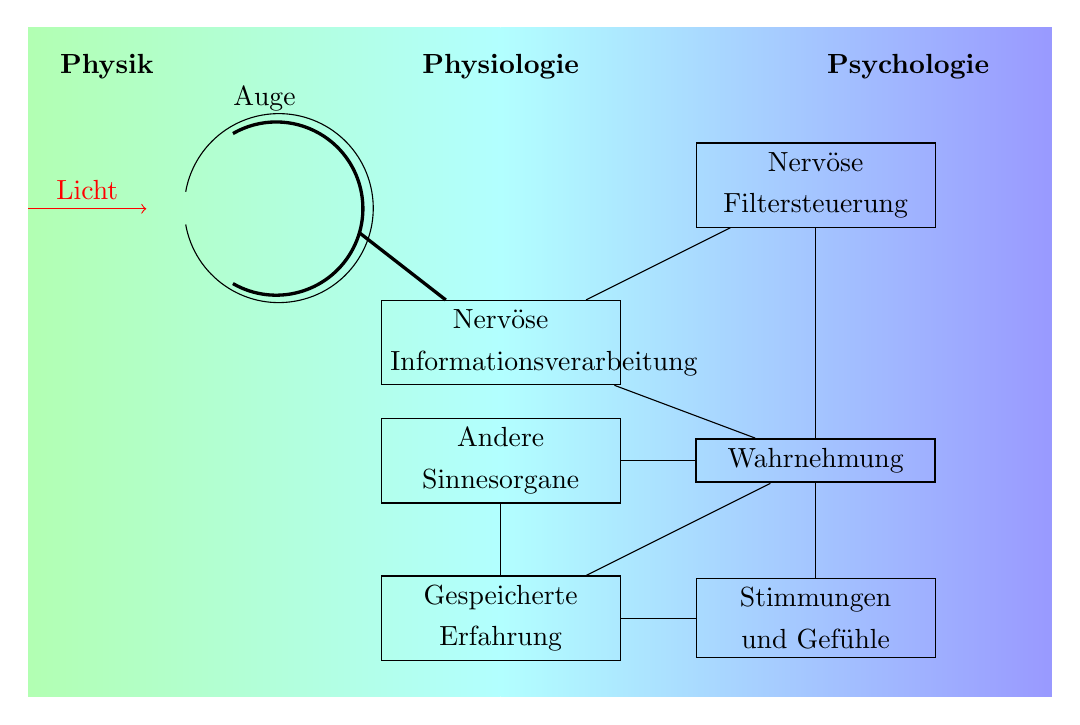
\begin{tikzpicture}[first style/.style={rectangle, rounded corners, align=center}, steuer style/.style={draw, rectangle, text width=2.8cm, align=center}]
	\shade[left color=cyan!30!white, right color=blue!40!white] (1, 5.5) rectangle (8,-3);
	\shade[left color=green!30!white, right color=cyan!30!white] (-5, 5.5) rectangle (1,-3);
	\draw (-3, 3) arc (-170:170:12mm);
	\draw[very thick] (-2.4, 2.25) arc (-120:120:11mm) ;
	\draw[->, red] (-5, 3.2) -- node[above] {Licht} (-3.5 , 3.2);
	\node[first style] (A) at (-2, 4.6) {Auge};
	\node[first style, ultra thick] (P1) at (-4, 5){\textbf{Physik}};
	\node[first style, ultra thick] (P2) at (1, 5){\textbf{Physiologie}};
	\node[first style, right=of P2, ultra thick] (P3) at (4, 5) {\textbf{Psychologie}};
	\node[steuer style] (S6) at (5, 3.5) {Nervöse Filtersteuerung};
	\node[steuer style, thick] (S1) at (5, 0) {Wahrnehmung};
	\node[steuer style] (S5) at (1, 1.5) {Nervöse Informationsverarbeitung};
	\node[steuer style] (S2) at (5, -2)  {Stimmungen und Gefühle};
	\node[steuer style] (S4) at (1, 0) {Andere Sinnesorgane};
	\node[steuer style] (S3)  at (1, -2) {Gespeicherte Erfahrung};
	\draw[very thick] (S5) -- (-0.8, 2.9);
	\draw (S1) -- (S2);
	\draw (S1) -- (S3);
	\draw (S1) -- (S4);
	\draw (S1) -- (S5);
	\draw (S1) -- (S6);
	\draw (S5) -- (S6);
	\draw (S2) -- (S3);
	\draw (S4) -- (S3);
\end{tikzpicture}
	\caption[Visuelle Wahrnehmung]{Visuelle Wahrnehmung}
	\label{fig:information}
\end{figure}

Ein bekanntes Beispiel für das Zusammenwirken zwischen den Sinnen, ist die Ausrichtung der Augen und des Kopfes durch das Hören von besonderen Geräuschen, wie einer Explosion.\\
Das bedeutet, dass die Wahrnehmung ganzheitlich betrachtet werden muss, da die einzelnen Wahrnehmungsarten miteinander in Wechselwirkung stehen. \\
Mit Medien können visuelle, auditive, haptische, motorische und olfaktorische Sinneskanäle angesprochen werden. Das Ziel der Medien ist dabei die Aufmerksamkeit des Menschen auf das Objekt zu richten und den erwünschten Einfluss auf den Menschen zu schaffen. Visuelle Inhalte können Schriften, Grafiken, Animationen oder Farben sein. Auditive sind Musik oder Geräusche. Haptische Inhalte sind fühlbare Strukturen und Oberflächen, während motorische Inhalte bewegliche Teile sind. Olfaktorische Reize sind Düfte und Gerüche. \cite[Vgl. Seite 3]{Buhler.2017}\\
In den nächsten Unterkapiteln werden die unterschiedlichen menschlichen Wahrnehmungsarten vertieft erläutert. Der Fokus ist auf die visuelle Wahrnehmung gerichtet, da dort der Schwerpunkt der späteren Arbeit liegt. Zu allen Wahrnehmungen wird auf die Physiologie der Sinne eingegangen und für diese Arbeit relevante Details.
\subsection{Visuelle Wahrnehmung}
Die visuelle Wahrnehmung basiert hauptsächlich auf den Sinneseindrücken durch unser Auge und daneben, wie oben erwähnt, aus dem Zusammenspiel der anderen Sinnesorgane. \\
Das Auge besitzt lichtempfindliche Zellen. Die Zellen werden dabei zwischen Stäbchen und Zapfen unterschieden. Die Mehrzahl an Zellen bilden die spektral unempfindlichen Stäbchen, mit ca. 120 Millionen pro Auge, während nur eine geringe Anzahl von 7 Millionen pro Auge farbempfindliche Zapfen sind. Durch den Unterschied in der Anzahl ist zum Beispiel das Sehen bei Dunkelheit eher schwarz-weiß, da die Anzahl der Zapfen nicht ausreicht, um genügend Licht zu erhalten und ein Farbbild zu erzeugen. Dabei ist ein Zapfen immer nur für eine der drei licht Frequenzbereiche rot (langwellig), grün (mittelwellig) oder blau (kurzwellig) lichtempfindlich. Die Farben in der menschlichen Wahrnehmung sind daher ein Ergebnis der Signalverarbeitung der drei unterschiedlichen Zapfenarten. \cite[Vgl. Seite 14]{Buhler.2017}\\
Abbildung \ref{fig:Auge} zeigt eine schematische Darstellung eines Auges mit der Vergrößerung eines Teilbereiches. In dem Teilbereich sind die Stäbchen und Zapfen dargestellt. \\
\begin{figure}[]
	\centering
	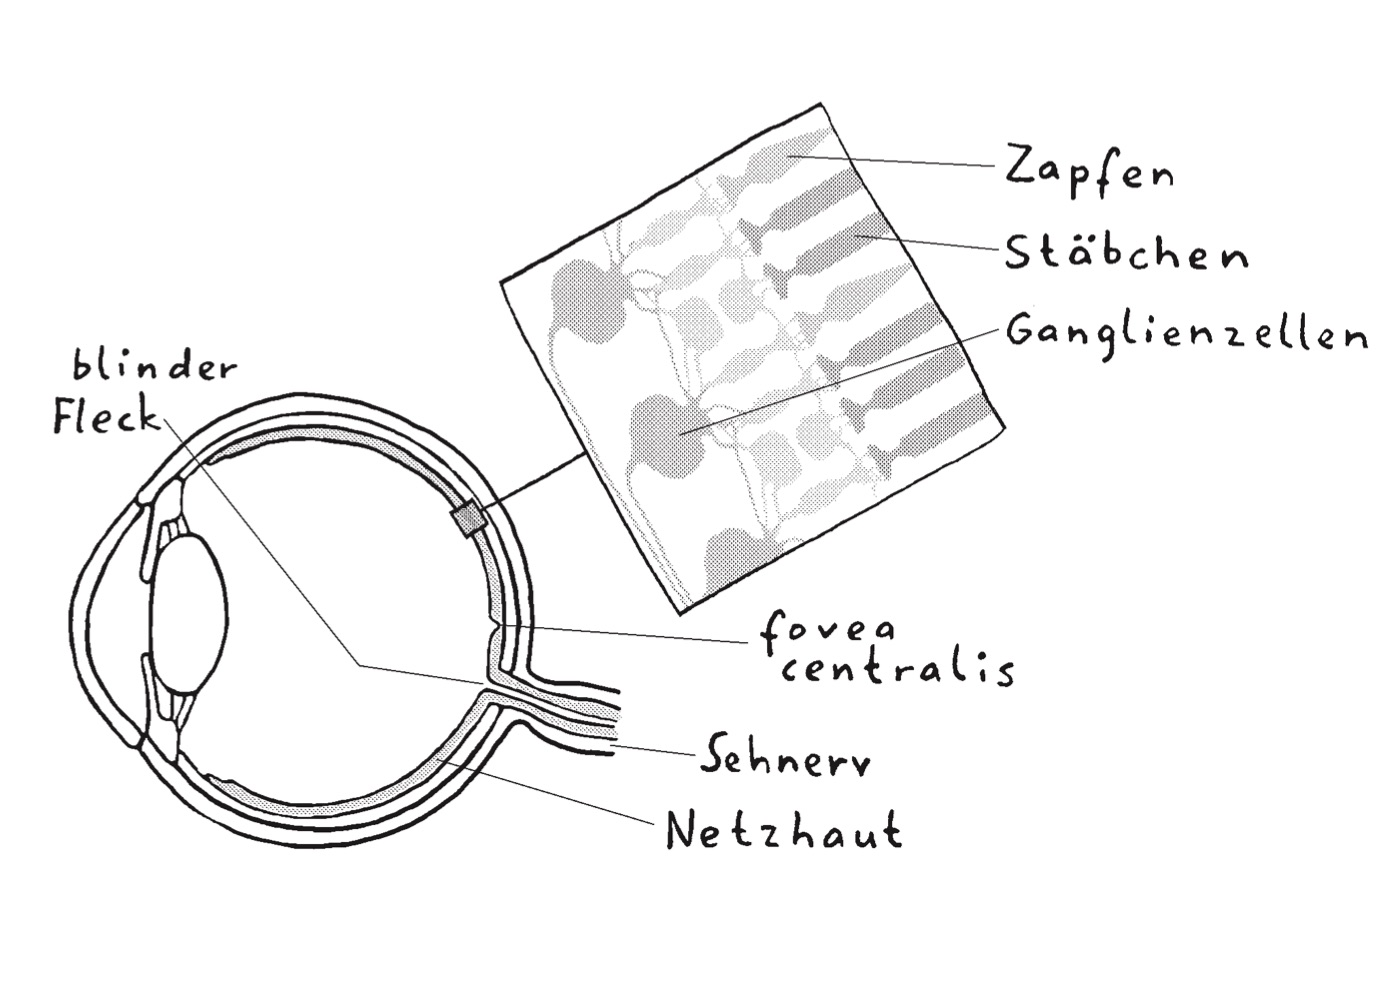
\includegraphics[width=0.5\linewidth]{images/Auge}
	\caption[Schematische Darstellung eines Auges mit den Nervenzellen]{Schematische Darstellung eines Auges mit den Nervenzellen \cite[Seite 141]{Schonhammer.2013}}
	\label{fig:Auge}
\end{figure}
Menschen können dabei nicht von ihrem Standpunkt aus den gesamten Raum betrachten, sondern durch biologischen Gegebenheiten immer nur ein eingeschränktes Feld. Das Blickfeld deckt in der Horizontalen ca. 180\,° und in der Vertikalen 120\,° ab. Von diesem Blickfeld sind nur ca. 1,5\,° in beiden Dimensionen als scharfes Bild sichtbar. \\
Durch Bewegungen des Auges und des Kopfes werden verschiedene scharfe Bereiche abgedeckt. Unser Gehirn fügt diese Bereiche zusammen, um ein ganzheitliches scharfes Blickbild zu erzeugen. \cite[Vgl. Seite 14]{Buhler.2017} \\
Interessant für die Bewertung der optischen Komponenten ist das Sehvermögen des Auges, Pixel bei einer bestimmten Distanz noch zu erkennen. Das Auflösungsvermögen beschreibt den kleinsten Winkel zwischen zwei Punkten, die noch als getrennt wahrgenommen werden. In der Literatur wird das Auflösungsvermögen $ A $\nomenclature{A}{Auflösungsvermögen} des menschlichen Auges auf $ 1' = \frac{1}{3000}\,^\circ = 0,0167\,^\circ $ angegeben. Mithilfe von trigonometrischen Rechnungen kann der Abstand $ x $ der zwei Punkte bei einer bestimmten Entfernung $ d $ und die dazu gehörige Pixeldichte $ P $ in ppi (pixel per inch\nomenclature{ppi}{pixel per inch}) berechnet werden. Die Bezugslänge $ d_{i} $ für die Pixeldichte ist häufig ein Inch. \cite[Vgl. Seite 209 f.]{LofflerMang.2020} \\
Als ein Bewertungskriterium von zweidimensionalen Anzeigen dient die Pixeldichte. Die Pixeldichte beschreibt, wie viele einzelne LEDs in einer bestimmten Richtung vorhanden sind. Je näher der Betrachter an der Anzeigefläche steht, desto höher muss die Pixeldichte sein, damit der Betrachter einzelne Pixel nicht erkennt. Bei Bildschirmen besteht die Möglichkeit, dass die Pixeldichte in die Höhe und in die Breite unterschiedlich ist. Wenn dies der Fall ist, wird häufig die Pixeldichte in diagonaler Richtung bestimmt. Die Skizze \ref{fig:Rechnung} beschreibt die Zusammenhänge der genannten Größen. \\
\begin{figure}[hbt]
	\centering
	\begin{tikzpicture}[first style/.style={rectangle, draw, rounded corners, align=center}, steuer style/.style={draw, rectangle, align=center}, second/.style={draw, rectangle, align=center, text width=3cm}]
	\draw (0,0) -- (5,0) -- node[right] {$ x $} (5, 0.5) -- node[above] {$ d $}(0,0);
	\draw (1.1, 0) arc (0:8:8mm);
	\node[] (S) at (1, -1) {$ \sin(A) = \frac{x}{d} $};
	\draw[->] (S) --(0.8, 0.05);
	\draw[<->] (5.5,0) -- node[right] {$ d_{i} $} (5.5,2);
\end{tikzpicture}
	\caption[Skizze zur Berechnung der Pixeldichte]{Skizze zur Berechnung der Pixeldichte}
	\label{fig:Rechnung}
\end{figure}
\begin{align}
	x &= \sin (A) \cdot d \\
	P &= \frac{d_{i}}{x}
\end{align}

Die Tabelle \ref{tab:Aufloessung} bildet eine Aufstellung über die Entfernung zwischen dem Auge und der Oberfläche mit der benötigten Pixeldichte.
\begin{table}[hbt]	
	\centering
	\renewcommand{\arraystretch}{1.5}	% Skaliert die Zeilenhöhe der Tabelle
	\captionabove[Berechnung der benötigten Pixeldichte bei einer bestimmten Entfernung]{Berechnung der benötigten Pixeldichte bei einer bestimmten Entfernung}
	\label{tab:Aufloessung}
	\begin{tabular}{l|r}
		\parbox[t]{0.2\linewidth}{\centering Entfernung} & \parbox[t]{0.2\linewidth}{\centering Pixeldichte}  \\
		\hline 
		\hline 
		$ 0,3\,\mathrm{m} $ & $ 291\,\mathrm{ppi} $ \\
		$ 0,5\,\mathrm{m} $ & $ 175\,\mathrm{ppi} $ \\
		$ 1,0\,\mathrm{m} $ & $ 87\,\mathrm{ppi} $ \\
		$ 2,0\,\mathrm{m} $ & $ 44\,\mathrm{ppi} $ \\
		$ 3,0\,\mathrm{m} $ & $ 29\,\mathrm{ppi} $ \\
		$ 5,0\,\mathrm{m} $ & $ 17\,\mathrm{ppi} $ \\
		$ 8,0\,\mathrm{m} $ & $ 11\,\mathrm{ppi} $ \\
		$ 10\,\mathrm{m} $ & $ 9\,\mathrm{ppi} $ \\
	\end{tabular} 
\end{table}
%\cite[Vgl. Seite 142 ff.]{Schonhammer.2013}%
\subsection{Haptische Wahrnehmung}
Die haptische Wahrnehmung ist ein Teilbereich der Somatosensorik. Die Sinneszellen der Somatosensorik werden in drei Bereiche eingeteilt:
\begin{itemize}
	\item Exterozeption, Wahrnehmung der Außenwelt
	\item Propriozeption, Wahrnehmung der Stellung der Gliedmaßen
	\item Interozeption, Wahrnehmung des inneren Körpers
\end{itemize}
Die somatosensorische Wahrnehmung verbindet diese drei Arten, die zum Teil bewusst oder unbewusst vom Körper aufgenommen werden. Besonders relevant für diese Arbeit im Bereich der haptischen Wahrnehmung ist die Exterozeption beziehungsweise die Oberflächensensibilität. \cite[Vgl. Seite 26]{Sprenger.2020}\\
Die haptische Wahrnehmung erfolgt durch Rezeptoren in der Haut, die die Form, Oberfläche und Position von Objekten registrieren. Die Rezeptoren können unterschieden werden in
\begin{itemize}
	\item Thermorezeptoren für relative Temperaturunterschiede zur Körperbefindlichkeit, 
	\item Chemorezeptoren für Stoffe,
	\item Nozirezeptoren für starke Temperaturunterschiede oder Drücke bis zur Gewebeschädigung und
	\item Mechanorezeptoren für Empfindung von Oberflächen und Druck.
\end{itemize}
Die Mechanorezeptoren können wiederum in unterschiedliche Arten eingeteilt werden, die auf Druck, Berührung oder Vibration reagieren. \cite[Vgl. Seite 26 f.]{Sprenger.2020} \\
Eine Übersicht bietet die Grafik \ref{fig:hapWahrnehmung}. Oben sind die unterschiedlichen Rezeptoren für die haptische Wahrnehmung zu sehen, während unten die Einteilung der Sinneszellen in die unterschiedlichen Wahrnehmungsarten erfolgt.
\begin{figure}[hbt]
	\centering
	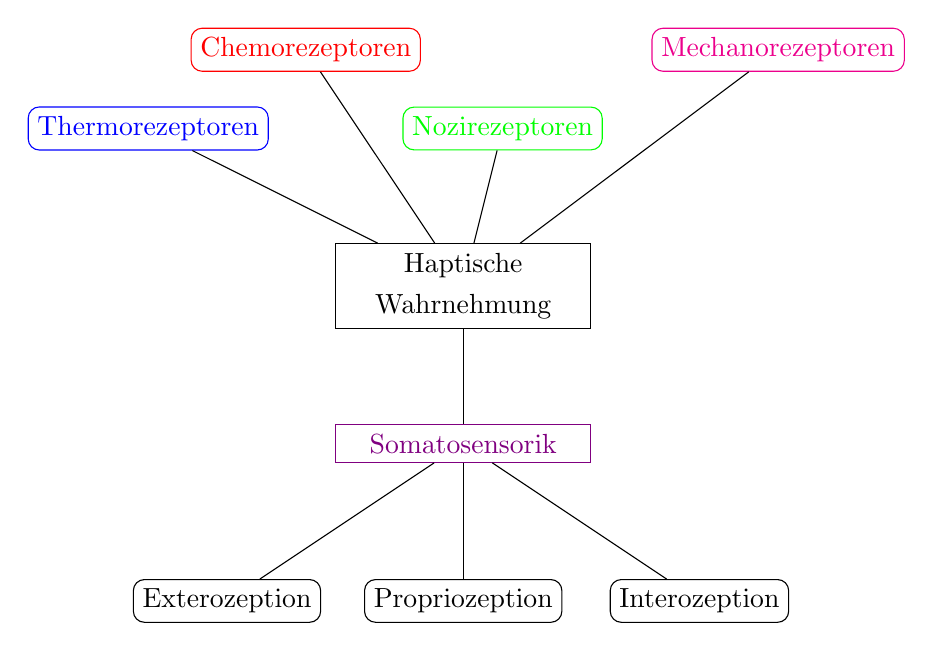
\begin{tikzpicture}[first style/.style={rectangle, draw, rounded corners, align=center}, steuer style/.style={draw, rectangle, text width=3cm, align=center}]
	\node[steuer style] (S1) at (0, 0) {Haptische Wahrnehmung};
	\node[steuer style, violet] (S2) at (0, -2) {Somatosensorik};
	\node[first style] (S3) at (-3, -4) {Exterozeption};
	\node[first style] (S4) at (0, -4) {Propriozeption};
	\node[first style] (S5) at (3, -4) {Interozeption};
	\node[first style, blue] (S6) at (-4, 2) {Thermorezeptoren};
	\node[first style, red] (S7) at (-2, 3) {Chemorezeptoren};
	\node[first style, green] (S8) at (0.5, 2) {Nozirezeptoren};
	\node[first style, magenta] (S9) at (4, 3) {Mechanorezeptoren};
	\draw (S1) -- (S2);
	\foreach \y in {3,...,5}
	\draw (S2) -- (S\y);
	\foreach \x in {6,...,9}
	\draw (S1) -- (S\x);
\end{tikzpicture}
	\caption[Haptische Wahrnehmung]{Haptische Wahrnehmung}
	\label{fig:hapWahrnehmung}
\end{figure}
Die Verteilung der unterschiedlichen Rezeptoren ist im Körper ungleichmäßig. In der Handinnenflächen gibt es zum Beispiel Areale mit unterschiedlicher Empfindsamkeit \glqq auf Druckintensität, Geschwindigkeit einer Veränderung an der Haut oder einer Vibration.\grqq{} \cite[Seite 29]{Sprenger.2020}\\
Die Empfindungsschwelle gibt Auskunft darüber, wie stark eine Hautstelle gedrückt werden muss, damit eine Berührung wahrgenommen wird. Durch das Berühren der Haut mit zwei Tastpunkten in bestimmter Entfernung kann das räumliche Auflösungsvermögen bestimmt werden. \cite[Vgl. Seite 28]{Sprenger.2020}\\
Die Wahrnehmung von Oberflächen geschieht über alle Sinneseindrücke. Zuerst werden die Hauptmerkmale Oberflächenstruktur, wie glatt oder rau, wahrgenommen und die Größe des Objektes durch die visuelle Wahrnehmung erfasst und im zweiten Schritt die gefühlte Temperatur. \cite[Vgl. Seite 33]{Sprenger.2020}\\
Das folgende Zitat beschreibt deutlich die Relevanz der haptischen Wahrnehmung für eine multisensuelle Gesamtinszenierung. \\
\glqq Die Verknüpfung der haptischen Wahrnehmung mit projizierten Simulationen zeigt letztendlich den Wunsch nach Kombinationen zu multisensuellen Interfaces, die allerdings nicht mehr die audiovisuelle Wahrnehmung als strikt dominant betrachten und die haptische Wahrnehmung ausschließlich als unterstützenden Sinn zur verbesserten Immersion heranziehen. Über die Haptik sollen direkt und unabhängig von anderen Sinnen Informationen gegeben wie auch erfahren werden, die in Kombination mit den anderen Sinnen kräftigere Informationsträger sind und somit auch als multisensuelle Kombinationen erforscht werden. \grqq{} \cite[Seite 263]{Sprenger.2020}
\subsection{Akustische Wahrnehmung}
Der Mensch ist in der Lage mit den Ohren Schallwellen zwischen $ 20 $ und $ 20.000\,\mathrm{Hertz} $ zu hören. Schallwellen sind Druckwellen eines Mediums wie Luft oder Wasser in longitudinaler Richtung. Das bedeutet, die Druckamplitudenrichtung ist parallel zur Ausbreitungsrichtung. \cite[Vgl. Seite 217]{Schonhammer.2013} \\
\glqq Über den äußeren Gehörgang gelangt die Schallwelle zum Trommelfell. Die Schwingungen des Trommelfells werden über die Kette der drei Gehörknöchelchen (Hammer, Amboss, Steigbügel) an das ovale Fenster übertragen, dessen Membran die mit Flüssigkeit gefüllte Schnecke (Cochlea) abschließt. Die Cochlea ist ein schneckenförmiger Kanal, der in das überaus harte Felsenbein eingebettet ist und die Basilarmembran enthält. Schallschwingungen erregen eine längs dieser Membran entlang fortschreitende Welle. Durch diese Auslenkung der Basilarmembran werden die Haarzellen angesprochen, die in einem geometrischen Muster längs der Basilarmembran angeordnet sind und das Muster der Anregung an das Gehirn übertragen. \grqq{} \cite[Seite 71f.]{Bernstein.2019}
Das Bild \ref{fig:Ohr} zeigt einen schematischen Aufbau des Gehörgangs mit den oben beschriebenen Teilen.
\begin{figure}[hbt]
	\centering
	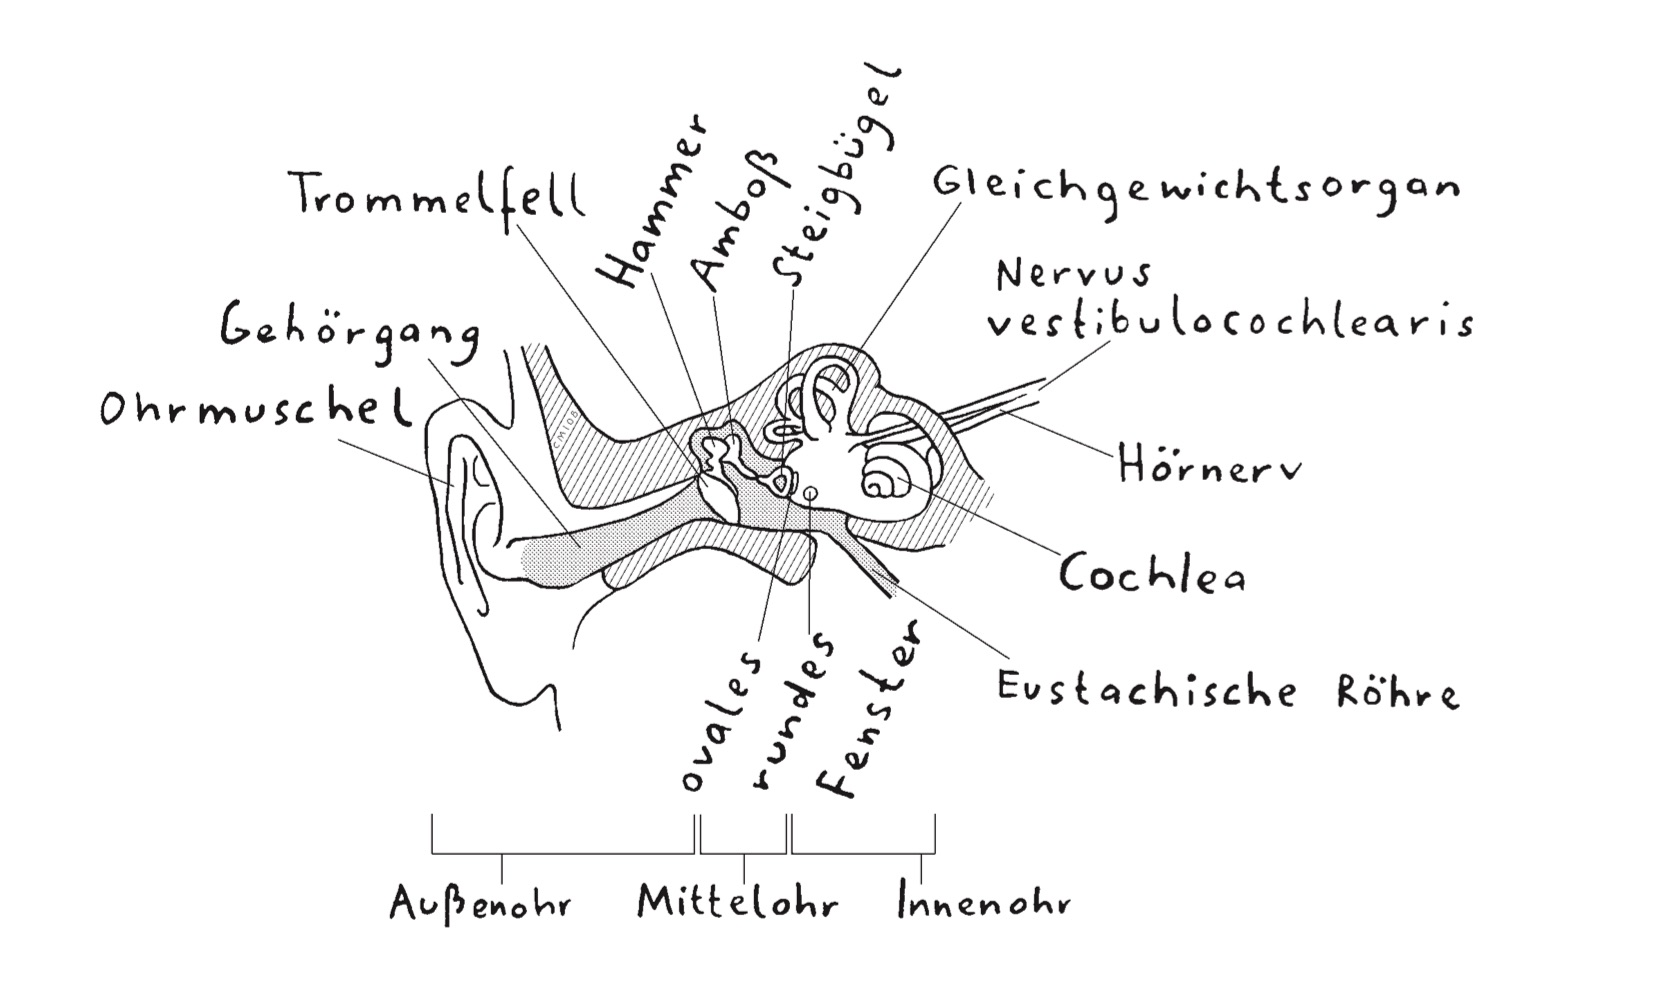
\includegraphics[width=0.7\linewidth]{images/Ohr}
	\caption[Schematische Darstellung des Gehörgangs mit den unterschiedlichen Bereichen]{Schematische Darstellung des Gehörgangs mit den unterschiedlichen Bereichen \cite[Seite 219]{Schonhammer.2013}}
	\label{fig:Ohr}
\end{figure}
\subsection{Olfaktorische Wahrnehmung}
Unser Körper ist in der Lage Gerüche schon bei sehr geringen Konzentrationen zu unterscheiden und Unterschiedlichkeiten wahrzunehmen. In der menschlichen Nase befinden sich Riechzellen in der Riechschleimhaut. Durch chemische Reize in den Rezeptoren der Zellen werden spezifische Entladungsmuster an evolutionär ältere Gehirnareale und das limbische System gesendet. Das limbische System ist maßgeblich für die Emotionen des Menschen verantwortlich. \cite[Vgl. Seite 102]{Schonhammer.2013}\\
Gerüche werden oft nach dem Stoff benannt mit dem sie assoziiert werden. Der Begriff \glqq blumig\grqq{} beschreibt Gerüchen, die dem Geruch von Blumen ähneln. \cite[Vgl. Seite 29 ff.]{Keller.2019}
Diese Klassifikation bei Gerüchen ist dabei nicht eindeutig, da die Zuordnung von Gerüchen zu Objekten Überschneidungen mit anderen Gerüchen haben können. Eine bessere erste Differenzierung von Gerüchen in Kategorien ist die Bewertung von Gerüchen nach angenehm und unangenehm. Da die olfaktorische Wahrnehmung und Gefühle eng miteinander verbunden sind. Angenehme Gerüche verursachen eine positive Stimmung und eine anziehende Gestik. \cite[Vgl. Seite 105 f.]{Schonhammer.2013}\\
Paul Jellinek klassifiziert Gerüche auf einer zweidimensionalen Karte \ref{fig:Duft} zwischen süß - bitter und basisch - sauer. \cite[Vgl. Seite 104]{Schonhammer.2013} \\
\begin{figure}[]
	\centering
	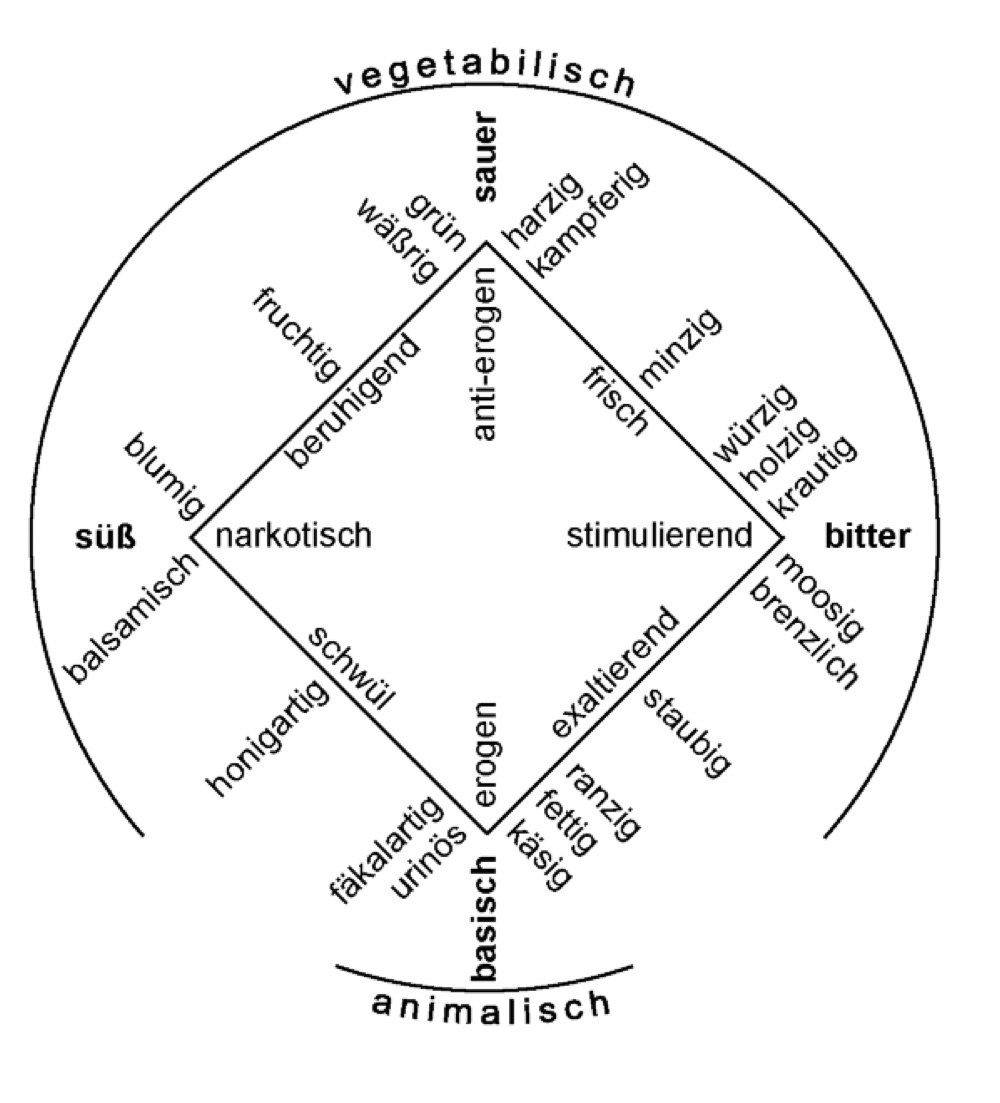
\includegraphics[width=0.5\linewidth]{images/Duft}
	\caption[Duftkreis nach P. Jellinek]{Duftkreis nach P. Jellinek \cite[Seite 105]{Schonhammer.2013}}
	\label{fig:Duft}
\end{figure}

Erste Überlegungen zur gesteuerten Stimulierung von Fahrzeuginsassen bildet das folgende Zitat:
\glqq Konzepte zur Beduftung der Innenräume von Automobilen werden u.a. unter dem Aspekt des allgemeinen Erregungszustandes des Fahrers vertreten. Gemeinsam mit Beleuchtung und Beschallung sollen Düfte den Menschen am Steuer etwa stimulieren oder beruhigen.\grqq{} \cite[Seite 122 f.]{Schonhammer.2013} \\
Dabei ist der Einsatz von Düften in Fahrzeugen stets behutsam anzuwenden. \\
\glqq Beduftung mag als verlockende Strategie emotional wirksamer Gestaltung erscheinen, ist jedoch nicht nur aus ethischen Gründen, sondern in Rücksicht auf das Wohlbefinden unfreiwillig Betroffener problematisch. [...] Schließlich ist daran zu erinnern, dass wegen der innigen Verbindung von Gefühl und Geruch Momente der visuellen, akustischen und taktil-haptischen Gestaltung indirekt auch auf das Riechen wirken. \grqq{} \cite[Seite 123]{Schonhammer.2013}
\section{Technologien}
In den folgenden Unterbereichen werden jeweils die einzelnen Technologien, die in dieser Arbeit behandelt werden, auf Funktionsweise, Beschaffenheit und Aufbau vorgestellt. Daneben werden die wichtigsten Kenngrößen zur Beurteilung der Technologien erläutert.
\subsection{Lumineszenzdiode}
Lumineszenzdioden (LED\nomenclature{LED}{Lumineszenzdiode}) sind lichtemittierende Dioden, die Strahlen im sichtbaren oder infraroten Spektralbereich erzeugen. Dioden sind die einfachste Form von elektronischen Bauteilen und bestehen aus dotierten Halbleitermaterial mit einer pn-Schicht. Das Halbleiter-Grundmaterial bestimmt den abgestrahlten Spektralbereich des Lichtes. Liegt eine Spannung in Durchlassrichtung der Dioden an, strahlt diese in ihrem Frequenzbereich Photonen ab. \cite[Vgl. Seite 193 f.]{LofflerMang.2020} \\
Die meisten LEDs sind SMD-Bauteile (Surface-mounted device\nomenclature{SMD}{Surface-mounted device}) und sitzen in einem Kunststoff-, Keramik- oder Epoxidharzgehäuse. Damit besitzen sie eine kompakte Bauform im Vergleich zu klassischen Glühbirnen. \\
Um eine Hintergrundbeleuchtung mit Hilfe von LEDs zu erzeugen kann ein Leuchtkörper mit einer Vielzahl an LEDs hinter einer Streulichtscheibe verbaut werden. Dadurch wird für eine homogene Darstellung eine geringe Pixeldichte benötigt. \cite[Vgl. Seite 194]{LofflerMang.2020} \\
Zum Erzeugen von weißem Licht strahlen drei verschiedene LEDs mit den Farben rot, grün und blau gleich hell. Erst im Auge entsteht durch die Kombination ein weißes Licht. Da hier aber drei LEDs genutzt werden, ist diese Variante teurer. Der Vorteil ist, dass bei variabler Einstellung der Helligkeit der einzelnen Dioden unterschiedliche Farben für den Betrachter angezeigt werden können. \\ 
Günstiger sind Weißlicht-LEDs (WLED\nomenclature{WLED}{Weißlicht-LED}), bei denen in der Produktion auf Basis von blauen LEDs noch ein fluoreszierender Konverterstoff beigemischt wird. Dieser Stoff wird durch das blaue Licht angeregt und strahlt einen breiten Spektralbereich wieder aus, wodurch ein weißes Licht aus Primär- und Sekundärlicht entsteht. Bei WLEDs ist die Farbe nicht variabel. \cite[Vgl. Seite 194]{LofflerMang.2020} \\
Organische LED (OLED\nomenclature{OLED}{Organische LED}) besitzen einen veränderten Schichtaufbau, bei dem zwischen p- und n-Schicht eine organische Schicht aufgebracht ist. OLEDs sind dünner als normale LEDs und dadurch leichter und flexibel, wodurch sich neue Einsatzbereiche ergeben. Daneben besitzen sie eine hohe Helligkeit bei starkem Kontrast. \cite[Vgl. Seite 195]{LofflerMang.2020}
\subsection{LED-Matrix}
Eine LED-Matrix ist eine bestimmte Anordnung von LEDs in zwei orthogonalen Richtungen auf einer Ebene. Somit entsteht ein zwei-dimensionales Bild. 
\subsection{Bildschirmtechnologien}
Unter den Bildschirmtechnologien werden folgend zwei unterschiedliche Realisierungen vorgestellt. Die erste Technologie sind aktive OLED-Displays und die zweite passive Flüssigkristallanzeigen (LCD\nomenclature{LCD}{Flüssigkristallanzeigen}). \\
Durch die schnellen Entwicklungen bei Bildschirmtechnologien ist es nicht möglich, alle unterschiedlichen Techniken vorzustellen. Die folgenden Absätze sollen ein Grundverständnis für die möglichen Funktionsweisen liefern.\\
Aktiv bedeutet in diesem Fall, dass die Pixel das Licht selbst erzeugen, während passive Displays auf ein Hintergrundlicht angewiesen sind, da sie nur Licht abdunkeln oder durchlassen können. \\
\glqq OLED-Displays bestehen aus einem zweidimensionalen Array weißes Licht abstrahlender OLEDs, denen Farbfilter (RGB) vorgelagert sind.\grqq \cite[Seite 347]{LofflerMang.2020} \\
Eine weitere Möglichkeit wären OLEDs mit unterschiedlichen Grundfarben (rot, grün und blau), die zusammen ein Pixel erzeugen. \\
Flüssigkristallanzeigen besitzen einen mehrschichtigen Aufbau. Die zentrale Schicht ist eine Flüssigkristallschicht, die bei Anlegen einer Spannung an den Elektrodenschichten der Flüssigkristalle ausrichtet und die Polarisierung des einfallenden Lichtes in eine bestimmte Richtung lenkt, sodass das Licht bei einem nachgeführten Polarisationsfilter entweder absorbiert oder transmittiert wird. \cite[][Vgl. Seite 346 f.]{LofflerMang.2020} \\
Je nach Ausführung kann das Licht bei angelegter Spannung oder spannungslos transmittieren. Die Richtung und Technik der Beleuchtung der LCD variiert je nach Herstellung.
\subsection{Videoprojektoren}
Videoprojektoren können auf Basis unterschiedlicher Technologien, die für differenzierte Situation angepasst sind, eingesetzt werden. Unterschiedliche Arten von Projektoren sind zum Beispiel LCD-, DLP- (Digital Light Processing\nomenclature{DLP}{Digital Light Processing}), LED-, LCoS- und Laser-Projektoren. \\
Zu Unterscheidung von Projektionsverfahren können diese wieder in aktive und passive Systeme eingeteilt werden. Heutzutage werden vorwiegend passive Systeme, sogenannte Lichtventilprojektoren, eingesetzt. \cite[Vgl. Seite 551]{Schmidt.2021} \\
Für die Auswahl des richtigen Projektors ist die Einsatzumgebung von Bedeutung. Je nach Helligkeit des Raumes ist die Helligkeit und der Kontrast unterschiedlich auszuwählen. Bei hoher Umgebungshelligkeit ist ein Projektor mit hoher Helligkeit vorzuziehen. Dabei ist ein niedrigerer Kontrast durch die Aufhellung der dunklen Bildbereiche durch das Umgebungslicht nicht negativ. \cite[Vgl. Seite 562]{Schmidt.2021}
\subsection{Elektronisches Papier}
Elektronisches Papier (E-Papier\nomenclature{E-Papier}{Elektronisches Papier}) ist eine Bezeichnung für Bildschirme, deren visuelle Anmutung Papier entspricht und deren Inhalt durch Elektronik gesteuert wird. Häufig sind diese Displays passiv, also reflektieren nur Licht und erzeugen keines. Bei manchen E-Papieren ist seitlich eine Hintergrundbeleuchtung, die über eine Folie das Display beleuchtet. Im folgenden wird die häufig verwendete Technologie der Elektrophorese für die Displays erläutert. \\
\glqq Elektronisches Papier lässt sich vereinfacht als dünne, flexible Folie beschreiben, in der in Flüssigkeit eingelagerte, elektrisch geladene Partikel (als elektronische Tinte bezeichnet) ein schwarz-weißes oder allgemein zweifarbiges Bild ergeben. Dies wird ermöglicht, indem über Elektroden elektrische Felder auf die Partikel wirken, die sich entsprechend der Ladung des angelegten Feldes ausrichten. \grqq{} \cite[Seite 568]{Schryen.2002} \\
\begin{figure}[]
	\centering
	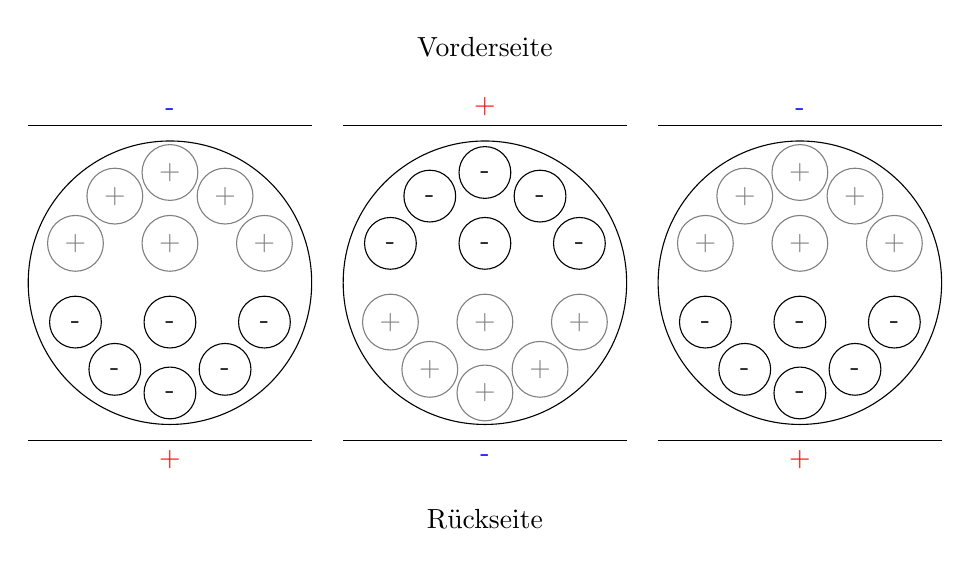
\begin{tikzpicture}[positiv/.style={circle, gray, draw, text width=0.3cm, align=center}, negativ/.style={circle, black, draw, text width=0.3cm, align=center}]
	\draw (0,0) circle [radius=1.8];
	\draw (-4,0) circle [radius=1.8];
	\draw (4,0) circle [radius=1.8];
	\draw (-1.8, 2) -- node[above, red] {+} (1.8, 2);
	\draw (-5.8, 2) -- node[above, blue] {-} (-2.2, 2);
	\draw (2.2, 2) -- node[above, blue] {-} (5.8, 2);
	\draw (-1.8, -2) -- node[below, blue] {-} (1.8, -2);
	\draw (-5.8, -2) -- node[below, red] {+} (-2.2, -2);
	\draw (2.2, -2) -- node[below, red] {+} (5.8, -2);
	\node[] (V) at (0, 3) {Vorderseite};
	\node[] (R) at (0, -3) {Rückseite};
	\node[positiv] at (0,-1.4) {$ + $};
	\node[positiv] at (-0.7,-1.1) {$ + $};
	\node[positiv] at (0.7,-1.1) {+};
	\node[positiv] at (0,-0.5) {+};
	\node[positiv] at (-1.2,-0.5) {+};
	\node[positiv] at (1.2,-0.5) {+};
	\node[negativ] at (-4,-1.4) {-};
	\node[negativ] at (-4.7,-1.1) {-};
	\node[negativ] at (-3.3,-1.1) {-};
	\node[negativ] at (-4,-0.5) {-};
	\node[negativ] at (-5.2,-0.5) {-};
	\node[negativ] at (-2.8,-0.5) {-};
	\node[negativ] at (4,-1.4) {-};
	\node[negativ] at (4.7,-1.1) {-};
	\node[negativ] at (3.3,-1.1) {-};
	\node[negativ] at (4,-0.5) {-};
	\node[negativ] at (5.2,-0.5) {-};
	\node[negativ] at (2.8,-0.5) {-};
	\node[negativ] at (0,1.4) {-};
	\node[negativ] at (-0.7,1.1) {-};
	\node[negativ] at (0.7,1.1) {-};
	\node[negativ] at (0,0.5) {-};
	\node[negativ] at (-1.2,0.5) {-};
	\node[negativ] at (1.2,0.5) {-};
	\node[positiv] at (-4,1.4) {+};
	\node[positiv] at (-4.7,1.1) {+};
	\node[positiv] at (-3.3,1.1) {+};
	\node[positiv] at (-4,0.5) {+};
	\node[positiv] at (-5.2,0.5) {+};
	\node[positiv] at (-2.8,0.5) {+};
	\node[positiv] at (4,1.4) {+};
	\node[positiv] at (4.7,1.1) {+};
	\node[positiv] at (3.3,1.1) {+};
	\node[positiv] at (4,0.5) {+};
	\node[positiv] at (5.2,0.5) {+};
	\node[positiv] at (2.8,0.5) {+};
\end{tikzpicture}
	\caption[Schichtaufbau eines E-Papiers]{Schichtaufbau eines E-Papiers}
	\label{fig:epapier}
\end{figure}
Pro Pixel eines Bildes wird eine Mikrokapsel genutzt in der sich mehrere positiv geladene weiße Partikel und negativ geladene schwarze Partikel befinden. Auf beiden Seiten der Folie befinden sich Elektroden, wovon eine auf der Betrachtungsseite transparent ist. Wird auf der transparenten Elektrode eine negative Spannung und auf der inneren Elektrode eine positive, richten sich die Mikrokapseln dementsprechend aus, dass die positiven Partikel nach außen zeigen. Das Bild ist dementsprechend weiß. \cite[Vgl. Seite 567 f.]{Schryen.2002} \\
Die Abbildung \ref{fig:epapier} zeigt den Schichtaufbau eines E-Papiers.\\
E-Papiere benötigen nur beim Ändern der Polarität der Pixel elektrische Energie, wodurch der Strombedarf bei seltene Bildschirmänderungen gering ist. \\
Vorteile gegenüber LCD-Displays sind die niedrigeren Herstellungskosten, geringeres Gewicht und die bessere Lesbarkeit. \cite[Vgl. Seite 569]{Schryen.2002} \\
Da bei E-Papieren vorwiegend Bilder dargestellt werden, soll im folgenden die Berechnung der Dateigröße eines Bildes für ein mögliches E-Papier erläutert werden.
\paragraph{Berechnung der Datengröße eines Bildes}
Zur Berechnung der Datengröße eines Bildes kann die Rohdatenmenge für jeden Pixel herangezogen werden. Jedes Pixel benötigt Informationen, wie es leuchten soll. Bei schwarz-weiß Displays benötigt ein Pixel nur die Information wie stark es leuchten soll, bzw. wie stark abdunkeln. Bei farbigen Displays werden für die drei Grundfarben Informationen benötigt. Diese Informationen werden als Farbtiefe bezeichnet. \\
Die Farbtiefe gibt an, wie viele unterschiedliche Farben gespeichert werden können. Bei einer Farbtiefe von $ 8\,\mathrm{Bit} $ können 256 unterschiedliche Farben dargestellt werden. Je größer die Farbtiefe desto höher ist die Datenmenge. Die Farbtiefe sollt danach ausgelegt werden, welche Farbqualität für ein Bild gewünscht ist und welche Genauigkeit das Anzeigemedium zur Verfügung stellt.
Die Rohdatenmenge ist das Produkt aus der Anzahl der Pixel und der Farbtiefe. \cite[Vgl. Seite 297 f.]{Stotz.2019}\\
Durch Algorithmen kann diese Datenmenge komprimiert werden, indem Informationen gelöscht werden, die eine Geringe Relevanz für die Betrachter besitzen, oder strukturelle Wiederholungen im Datenspeichersatz gekürzt werden. Die Datenkompression kann je nach Kompressionsalgorithmus eingeteilt werden in verlustbehaftete und verlustfreie Kompression. Bei einer verlustfreien Kompression kann das originale Bild aus dem Komprimierten wiederhergestellt werden, was bei verlustbehafteten Kompression nicht der Fall ist. \\
Kompression benötigt für eine Dateneinsparung Rechenleistung bei der Kompression und Dekompression. Deswegen ist abzuwägen, wie stark die Datenkompression bei Daten eingesetzt werden soll. \\
Als Beispiel dient ein Schwarz-Weiß E-Papier mit einer Farbtiefe von 16 Stufen. Die Farbtiefe $ FT $\nomenclature{FT}{Farbtiefe} beträgt bei 16 Stufen zwar nur 5 Bit, um aber auf gängige Datengrößen zu kommen, sollte für die Berechnung 8 Bit pro Pixel und damit 1 Byte angenommen werden. Das Dateiformat JPEG \nomenclature{JPEG}{Joint Photographic Experts Group} nutzt 8 Bit pro Farbkanal. Die Pixelanzahl pro Zeile $ P $ \nomenclature{P}{Pixelanzahl pro Zeile}beträgt 1920 Pixel und Zeilenanzahl $ Z $\nomenclature{Z}{Zeilenanzahl} 1080 Pixel. Für den Komprimierungsfaktor $ KF $\nomenclature{KF}{Komprimierungsfaktor} wird hier ein Mittelwert von 12 angenommen. \cite[Vgl. Seite 22]{Buhler.2018}
\begin{align}
		Datenmenge &= \frac{P \times PZ \times FT}{KF} \label{eq:Bilddatenmenge}\\
		&= \frac{1920\,\frac{\mathrm{Pixel}}{\mathrm{Zeile}}\times 1080\,\mathrm{Zeilen} \times 8\,\frac{\mathrm{Bit}}{\mathrm{Pixel}}}{12} \\
		&= 1.382.400\,\mathrm{Bit} = 1,3824\,\mathrm{MBit} = 172,8\,\mathrm{KByte}
\end{align}
\section{Bordnetz}
Zur Kommunikation zwischen Steuergeräten von Fahrzeugkomponenten werden unterschiedliche Bussysteme genutzt. \\
Im folgenden werden die gängigen Bussysteme in der Fahrzeugtechnik vorgestellt, um für den späteren Konzeptentwurf die notwendigen Grundlagen zu kennen. Im Anschluss erfolgt ein Vergleich zwischen den Merkmalen der einzelnen Bussysteme. \cite[Vgl. Seite 124 ff.]{Schauffele.2016}
\subsection{Controller Area Network (CAN)}
CAN\nomenclature{CAN}{Controller Area Network} wird zum Austausch von Mess-, Steuer- und Regelsignalen genutzt. Es ist ein bitstrom-orientiertes System. Es basiert auf Differenzsignalübertragung und benutzt dazu verdrillte Leiterpaare. Als ereignisgesteuertes System wird das Senden von Nachrichten durch ein Ereignis ausgelöst. \cite[Vgl. Seite 15 ff.]{Wolf.2018}\\
Der High-Speed CAN besitzt Bitraten von $ 250\,\frac{\mathrm{kBit}}{\mathrm{s}} $ bis zu $ 1\,\frac{\mathrm{MBit}}{\mathrm{s}}$.
Der Low-Speed CAN besitzt Bitraten kleiner als $ 125\,\frac{\mathrm{kBit}}{\mathrm{s}} $. 
Der CAN verfügt über Fehlererkennung und Sicherungssysteme. Das Senden von Nachrichten erfolgt über eine Priorisierung der Nachrichten. \cite[Vgl. Seite 57 ff.]{Zimmermann.2014}
\paragraph{Performance}
Je nach Ausschöpfung der Nutzdatenmenge pro Botschaft liegt die maximale Übertragungsgeschwindigkeit zwischen $ 7,7\,\frac{\mathrm{kByte}}{\mathrm{s}} $ bei einem Byte Nutzdaten pro Botschaft und $ 29,6\,\frac{\mathrm{kByte}}{\mathrm{s}} $ bei acht Byte Nutzdaten. Die Latenz einer Botschaft ist nicht deterministisch bestimmbar und ist abhängig von der aktuellen Buslast und der Priorität der Botschaft. Die Übertragungsdauer einer Botschaft mit maximaler Nutzdatenmenge bei $ 500\,\frac{\mathrm{kBit}}{\mathrm{s}} $ Bittakt liegt bei $ 270\,\mathrm{\mu s}$.
Durch den Einsatz der weiterentwickelten CAN-Version CAN FD (CAN with Flexible Data Rate\nomenclature{CAN FD}{CAN with Flexible Data Rate}) kann die Übertragungsgeschwindigkeit durch größere Nutzdatenmengen und höherer Bittakte auf bis zu $ 260\,\frac{\mathrm{kByte}}{\mathrm{s}} $ gesteigert werden. \cite[Vgl. Seite 76 ff.]{Zimmermann.2014}
\subsection{Local Interconnect Network (LIN)} 
Der LIN\nomenclature{LIN}{Local Interconnect Network} soll mit einem einfacheren Aufbau eine kostengünstige Alternative zum CAN für Low Speed Sensor-Aktor Anwendungen bieten. \cite[Vgl. Seite 138 ff.]{Borgeest.2021}
LIN ist ein Master-Slave gesteuertes Netzwerk, worin der Master die gesamte Kommunikation steuert, indem er die Slaves nach einem Zeitplan Berechtigungen zum Senden gibt. Die Bitrate beträgt üblicherweise $ 19,2\,\frac{\mathrm{kBit}}{\mathrm{s}} $. \cite[Vgl. Seite 79 ff.]{Zimmermann.2014}
\paragraph{Performance}
Für Botschaften mit acht Byte Nutzdaten werden Sendezeitraster von $ 10\,\mathrm{ms} $ benötigt. Die Nutzdatenmenge beträgt dementsprechend ca. $ 800\,\frac{\mathrm{Byte}}{\mathrm{s}} $. \cite[Vgl. Seite 94 f.]{Zimmermann.2014}
\subsection{FlexRay}
Mit dem Hintergrund, dass bei CAN keine deterministischen Aussagen zur Latenz getroffen werden können, wurde der FlexRay zum Austausch zeitkritischer Mess-, Steuer- und Regelsignalen mit hoher Fehlersicherheit entwickelt. Die Bitraten beim FlexRay betragen zwischen $ 2,5\,\frac{\mathrm{MBit}}{\mathrm{s}} $ und $ 10\,\frac{\mathrm{MBit}}{\mathrm{s}} $.
\cite[Vgl. Seite 96 ff.]{Zimmermann.2014}
\paragraph{Performance}
Die Nutzdatenmenge beträgt je nach Bitrate $ 1000\,\frac{\mathrm{kByte}}{\mathrm{s}} $ pro Kanal bei einem Bittakt von $ 10\,\frac{\mathrm{MBit}}{\mathrm{s}} $. \cite[Vgl. Seite 118 f.]{Zimmermann.2014}
\subsection{Media Oriented Systems Transport (MOST)}
MOST ist für Telematik- und Multimedia- Anwendungen mit hohen Übertragungsbandbreiten konzipiert.
Die Botschaften werden dabei nach Kanälen, in denen sich Audio-, Video- oder andere Daten befinden, gruppiert.
Die Bitraten betragen in unterschiedlichen Stufen $ 25\,\frac{\mathrm{MBit}}{\mathrm{s}} $, $ 50\,\frac{\mathrm{MBit}}{\mathrm{s}} $ und $ 150\,\frac{\mathrm{MBit}}{\mathrm{s}} $.
\paragraph{Performance}
Nutzdatenrate liegt bei MOST25 bei $ 2,6\,\frac{\mathrm{MByte}}{\mathrm{s}} $, MOST50 $ 5,6\,\frac{\mathrm{MByte}}{\mathrm{s}} $  und MOST150 bei $ 17,8\,\frac{\mathrm{MByte}}{\mathrm{s}} $.
\cite[Vgl. Seite 119 ff.]{Zimmermann.2014}
\subsection{Automotive Ethernet}
Automotive Ethernet ist standardisiert in der IEEE 802.3 und basiert auf dem normalen Ethernet Protokoll. Der Unterschied besteht im Nutzen von einem Paar ungeschirmt verdrillte Drahtleitungen durch eine
\paragraph{Performance}
Es sind bis zu 1500 Byte Nutzdaten pro Frame möglich. Es ergibt sich eine maximal mögliche Nutzdatenmenge bei einem Bittakt von $ 10\,\frac{\mathrm{MBit}}{\mathrm{s}} $ von ca. $ 10\,\frac{\mathrm{MByte}}{\mathrm{s}} $. \cite[Vgl. Seite 138 ff.]{Zimmermann.2014}
\subsection{Vergleich der einzelnen Bussysteme}
Im folgenden werden die oben vorgestellten Bussysteme miteinander verglichen in Tabelle \ref{tab:Bussysteme} anhand der Bittakt- und Nutzdatenrate.
\begin{table}[hbt]	
	\centering
	\renewcommand{\arraystretch}{1.5}	% Skaliert die Zeilenhöhe der Tabelle
	\captionabove[Vergleich der Bittakt- und Nutzdatenraten der Bussysteme]{Vergleich der Bittakt- und Nutzdatenraten der Bussysteme}
	\label{tab:Bussysteme}
	\begin{tabular}{l|rr}
		 \parbox[t]{0.2\linewidth}{\centering Bussystem} & \parbox[t]{0.2\linewidth}{\centering Bittakt} & \parbox[t]{0.2\linewidth}{\centering Nutzdatenrate}  \\ 
		\hline 
		\hline
		LIN & $ 19,2\,\frac{\mathrm{kBit}}{\mathrm{s}} $ & $ 0,8\,\frac{\mathrm{kByte}}{\mathrm{s}} $  \\
		CAN Low-Speed & $ 125\,\frac{\mathrm{kBit}}{\mathrm{s}} $ & $ 7,4\,\frac{\mathrm{kByte}}{\mathrm{s}} $ \\
		CAN High Speed & $ 500\,\frac{\mathrm{kBit}}{\mathrm{s}} $ & $ 29\,\frac{\mathrm{kByte}}{\mathrm{s}} $  \\
		FlexRay & $ 10.000\,\frac{\mathrm{kBit}}{\mathrm{s}} $ & $ 1.000 \,\frac{\mathrm{kByte}}{\mathrm{s}} $  \\
		MOST25 & $ 25.000\,\frac{\mathrm{kBit}}{\mathrm{s}} $ & $ 2.600\,\frac{\mathrm{kByte}}{\mathrm{s}} $  \\
		MOST50 & $ 50.000\,\frac{\mathrm{kBit}}{\mathrm{s}} $ & $ 5.600\,\frac{\mathrm{kByte}}{\mathrm{s}} $  \\
		MOST150 & $ 150.000\,\frac{\mathrm{kBit}}{\mathrm{s}} $ & $ 17.800\,\frac{\mathrm{kByte}}{\mathrm{s}} $  \\
		Automotive Ethernet & $ 100.000\,\frac{\mathrm{kBit}}{\mathrm{s}} $ & $ 10.000\,\frac{\mathrm{kByte}}{\mathrm{s}} $  \\
	\end{tabular} 
\end{table}
\chapter{Fahrzeugprototyp}
\label{cha:Prototyp}
\section{Vision}
Das Gesamtkonzept für den Fahrzeugprototypen basiert auf der Vision eines \glqq Fahrzeuges als Leinwand\grqq{} (englisch: \glqq Car as a canvas\grqq{}). Das Zielbild dieser Vision ist ein Fahrzeug, das auf vollständiger Weise seine Wahrnehmung auf den Menschen verändern kann. Besonders die visuelle Wahrnehmung ist hier im Vordergrund der Vision, aber diese bleibt nicht singulär, sondern die anderen Wahrnehmungsarten sollen die visuelle Wahrnehmung unterstützen.\\
Unter der übergeordneten Vision das Fahrzeug als Leinwand zu betrachten, bildet das Gesamtkonzept des Prototypen einen möglichen ersten Schritt in Richtung der Vision.
\section{Gesamtkonzept}
Das Gesamtkonzept besteht im Kern um digitale Kunst im Fahrzeug. Kunden können unterschiedliche digitale Kunstinhalte, sogenannte Kollektionen, erwerben und diese Kollektionen in ihrem Fahrzeug aktivieren. Die Kollektionen bestehen aus mehreren inhaltlichen Bestandteilen, welche auf neuartigen und bestehenden Fahrzeugkomponenten im Fahrzeug dargestellt werden. Die Darstellung der Inhalte der Kollektionen kann entweder durchgehend sein oder nur durch bestimmte Trigger wie zum Beispiel das Entriegeln der Türen ausgelöst werden.
Neben optischen Komponenten unterstützen haptische, olfaktorische und akustische Komponenten die Kollektionen. Dazu bilden Augmented Reality (AR\nomenclature{AR}{Augemented Reality}) Anwendungen weitere Darstellungen der Kollektionen mit Hilfe einer eigenen App auf einem Mobiltelefon.\\
Die App ist für den Besitzer das zentrale Steuersystem in der unterschiedliche Aktionen auf den einzelnen Seiten verfügbar sind:
\begin{itemize}
	\item Kollektionen können auf digitalen Börsen gehandelt werden
	\item Gekaufte Kollektionen können im Fahrzeug aktiviert werden oder durch AR auf dem Mobiltelefon gezeigt werden
	\item zusätzliche AR Inhalte zu den Kollektionen können auf dem Mobiltelefon gezeigt werden
	\item einzelne Komponenten der aktivierten Kollektion können deaktiviert werden
	\item über ein eigenes Profil kann mit anderen Besitzern von Kollektionen Bilder durch ein soziales Netzwerk ausgetauscht werden
\end{itemize}
Im Gegensatz zu bisherigen Individualisierungsmöglichkeiten, wie zum Beispiel Ambientebeleuchtung oder LED Scheinwerfer, können die Kollektionen in diesem Gesamtkonzept zum Einen dynamisch ihre Inhalte verändern und zum Anderen das gesamte Erscheinungsbild des Fahrzeuges durch ganzheitlich verändern. Daneben bietet das Gesamtkonzept ein Ökosystem für den Handeln und die Interaktion für Kollektionen als digitale Wertgegenstände.
\section{Beschreibung}
Der Prototyp wurde unter den Leitlinien des Gesamtkonzeptes entwickelt. Aufbauend auf einem produzierten elektrischen Serienfahrzeug wurden im Exterieur und Interieur Teile ergänzt und teilweise mit anderen Komponenten ausgetauscht, um das Gesamtkonzept zu folgen. Die Serienfunktionen wurden zum größten Teil durch die Umbauten nicht beeinträchtigt.\\
Durch Zeit- und Budgetknappheit besitzt das Fahrzeug nicht alle Ideen des Gesamtkonzeptes. Bei den Hardware Komponenten gibt es keine mit olfaktorischen Sinneseindrücken. Die App besitzt alle oben beschriebenen Funktionen zumindest als Schaubilder, aber hat nur die Auswahl und Steuerung der Kollektionen und AR Inhalte als Funktionen implementiert.
\section{Exterieur Komponenten}
Das Fahrzeug hat sowohl im Exterieur als auch im Interieur Komponenten verbaut. Zuerst werden die Komponenten im Exterieur und dann im Interieur vorgestellt. Die Komponenten wurden nach der verwendeten Technik und dem Ort benannt und nicht nach den Markennamen. Die Einteilung erfolgt nach der Betrachtungsweise innerhalb oder außerhalb des Fahrzeugs der Komponenten. Exterieur Komponenten werden von Beobachtern außerhalb des Fahrzeugs betrachtet. Interieur Komponenten entsprechend von innen.\\
Im Exterieur sind dies ein E-Papier in der Frontschürze, ein durchgehendes LED-Streifen in der Frontschürze, E-Papier Embleme über den beiden vorderen Radkästen, LED-Streifen in allen vier Radkästen, Videoprojektoren in den beiden Außenspiegel, nach außen gerichtete Bildschirme in den hinteren Seitenfenstern, ein LED-Streifen in der Heckleuchte und zwei kleine E-Papiere unterhalb der Heckleuchte.\\
Im folgenden werden alle Exterieur Komponenten nähe betrachtet:
\subsection{E-Papier in der Frontschürze}
Das E-Papier befindet sich hinter einer Scheibe mit einem Markenlogo in der Mitte der Fahrzeugfront und schließt an den Seiten über eine Abmaskierung auf die beiden Frontlichter an. Das E-Papier bewirkt mit der Laminierung an der Scheibe einen räumlichen Effekt, wonach das Markenlogo vor dem E-Papier hervor strahlt.
Auf dem E-Papier werden graphische Designs dargestellt, die Betrachter vor dem Auto sehen können.\\
Das E-Papier hat ein Format von 16:9 und eine Auflösung von $ 2560\times 1440 $, wovon ein teil des Bildschirms am Rand durch eine Abmaskierung nicht sichtbar ist.
\subsection{LED-Streifen in der Frontschürze}
Der LED-Streifen ist dreiteilig aufgeteilt. Die zwei äußeren Teile befinden sich in der Frontleuchten und schließen auf gleicher Höhe mit dem mittleren Streifen an. Der mittlere Streifen befindet sich oberhalb des E-Papier in der Frontschürze. \\
Auf dem Streifen werden dynamische bunte Lichtsequenzen gezeigt.
Zusammen mit dem E-Papier in der Frontschürze bilden diese zwei Komponenten die Darstellung der Kollektionen im Frontbereich.
Der mittlere Teil besitzt 130 Bildpunkte und die äußeren Teile 101 Punkte.
\subsection{E-Papier Embleme über den vorderen Radkästen}
Oberhalb der Radkästen befinden sich in einem ca. 20 cm breitem und 8 cm hohen Ausschnitt E-Papiere. An dieser Stelle befand sich vorher ein Emblem der Fahrzeugbezeichnung.
Die E-Papiere werden genutzt, um den Namen der verwendeten Kollektion anzuzeigen. \\
Die E-Papiere haben ein Format von 4:3 und eine Auflösung von $ 1600\times1200 $.
\subsection{LED-Streifen in den Radkästen}
In allen vier Radkästen befinden sich LED-Streifen am äußeren Rand und strahlen durch eine Leiste nur in den Radkasten Innenraum auf den oberen Halbkreis des Reifenprofils. 
Pro Radkasten befinden sich 196 LEDs. 
\subsection{Videoprojektoren in den Außenspiegeln}
In den Außenspiegeln wurde der Innenraum mit der Spiegelmechanik ausgebaut und Videoprojektoren eingebaut. Der nach unten ausgerichtete Videoprojektor bestrahlt die Flächen durch ein Loch an der Unterseite des Außenspiegels vor den vorderen Türen.
Durch den Videoprojektor können Videos auf dem Boden gezeigt werden.\\
Die Videoprojektoren haben ein Format von 16:10 und eine Auflösung von $ 1280\times800 $.
\subsection{Bildschirme in den hinteren Seitenfenstern}
In den hinteren Seitenfenstern befinden sich hinter der unbeweglichen Nebenscheiben, die mit einer Leiste von den beweglichen Hauptglasscheiben getrennt sind, Bildschirme. Diese können von außen betrachtet werden. Die Rückseite der Bildschirme ist von innen mit einer schwarzen Kunststoffverkleidung für die Passagiere abgedeckt.\\
Zusammen mit den LED-Streifen in den Radkästen und den Videoprojektoren in den Außenspiegeln bilden die Bildschirme in den Seitenfenstern die optische Darstellung der Kollektionen im Seitenbereich.
Die Bildschirme haben ein Verhältnis von 16:10 und eine Auflösung von $ 1280\times800 $.
\subsection{LED-Streifen in der Heckleuchte}
In der Serienheckleuchte wurde das rote Leuchtband mit einem LED-Streifen getauscht. Der Streifen ist dreigeteilt mit dem mittleren Teil in der Heckklappe und den zwei äußeren Teilen im hinteren Kotflügel. \\
Der mittlere Streifen besitzt 219 LED und die äußeren Streifen 86 LED.
\subsection{E-Papier in der Heckleuchte}
Direkt unterhalb der Heckleuchten sind zwei E-Papiere in der Heckklappe eingebaut.
Diese E-Papiere haben einen ähnlich großen Ausschnitt wie die E-Papiere oberhalb der Radkästen und werden auch genutzt, um den Namen der Kollektionen zu zeigen. Das Format und die Auflösung sind identisch zu diesen mit 4:3 und $ 1600\times1200 $\\
Zusammen mit dem LED-Streifen in der Heckleuchte bilden die E-Papiere die Heckansicht der Kollektion für Betrachter.
\section{Interieur Komponenten}
Im Interieur sind die Komponenten ein durchgehender LED-Streifen von den hinteren Türen über die vorderen Türen bis über das gesamte Cockpit, in den Türen ein LED Feld, Bildschirme in der Einstiegsleiste der vorderen Türen, Videoprojektoren im Fußraum der Frontsitze, Benutzeroberflächen für den Fahrer- und den Zentralbildschirm, eine morphende Oberfläche in der Mittelkonsole, einen durchsichtigen Bildschirm im Dachfenster und eine LED Matrix im Dachhimmel.\\
Daneben sind weitere Komponenten Duftflakons im Innenraum, Bildschirmoberflächen im Cockpit und ein Soundplayer im Innenraum.
Im folgenden werden alle Interieur Komponenten näher vorgestellt.
\subsection{LED-Streifen im Interieur}
Der LED-Streifen ist fünf geteilt und erstreckt sich im oberen Bereich der vier Türverkleidungen und schließt über das Cockpit zu einem einheitlichen Band ab. Der Streifen befindet sich hinter einer Streulichtscheibe, damit der Betrachter nicht die einzelnen LED erkennen kann. \\
Der Streifen spielt dynamische Inszenierungen für die Fahrzeuginsassen ab.
Die Leisten in den Türen haben eine Auflösung von 115 Pixel, während das mittlere Stück 259 Pixel besitzt.
\subsection{LED Türtafeln}
In allen vier Türverkleidungen befinden sich unterhalb des LED-Streifens ein LED Feld hinter einer Abdeckung mit durchsichtigen Sternen. Die Sterne können somit mit unterschiedlichen Farben angestrahlt werden.\\
\subsection{Bildschirme in der Einstiegsleiste}
Anstelle einer Edelstahl Abdeckung mit einem Schriftzug befinden sich in den vorderen Türen Bildschirme in der Einstiegsleiste. Die Bildschirme können bei geöffneter Türe Inhalte dem Fahrzeuginsassen und Betrachter Außerhalb des Fahrzeuges darstellen.\\
Die Auflösung der Bildschirme beträgt $ 1280\times1024 $.
\subsection{Videoprojektoren im Fußraum}
Für die vorderen Fußraumböden wurden zwei Videoprojektoren verbaut. Der linke Videoprojektor befindet sich unterhalb der Lenksäule, der rechte unterhalb des Handschuhfachs. Beide Videoprojektoren strahlen den Fußraum an und können dynamisch Inhalte abspielen.
Die Videoprojektoren haben ein Format von 16:10 und eine Auflösung von $ 1280\times800 $.
\subsection{Morphende Oberfläche in der Mittelkonsole}
In der Mittelkonsole wurde das Ablagefach und die abgelederte Abdeckung durch eine neuartige Vorrichtung ersetzt, die von innen mit Hilfe von Formteilen auf die Oberflüche drückt und somit von außen optisch und haptisch spürbar ist. In der Vorrichtung befinden sich in einem Revolver drei Formteile mit unterschiedlicher Ausgestaltung.
\subsection{Durchsichtiger Bildschirm im Dachfenster}
An das Dachfenster wurde ein durchsichtiges Bildschirm geklebt, das bei Betrachten von innen Grafiken darstellen kann.
Der Bildschirm ist Full HD mit einer Auflösung von $ 1920\times1080 $.
\subsection{LED Matrix im Dachhimmel}
Im Dachhimmel unter der Stoffverkleidung befindet sich eine LED Matrix. Das Feld kann dynamische Farbeffekte erzeugen.
Insgesamt besitzt die LED Matrix eine Auflösung von $ 192\times96 $.
\subsection{Duftflakons im Innenraum}
Im Innenraum befinden sich Duftflakons, die jeweils für eine bestimmte Kollektion erstellt wurden. Es ist kein technischer Aufbau zur automatischen Beduftung des Innenraumes vorhanden.
\subsection{Bildschirmoberflächen im Cockpit}
Das zentrale Kombiinstrument und das digitale Fahrerdisplays haben die Möglichkeit unterschiedliche Bildschirmoberflächen anzuzeigen.
\subsection{Soundplayer im Innenraum}
Das Soundsystem im Innenraum kann extern über den Zentralrechner angesteuert werden und MP3 Dateien abspielen.
\section{Ansteuerung}
Die Ansteuerung der Komponenten erfolgt über einen zentralen Rechner mit Windows Betriebssystem, der sich im Kofferraum des Fahrzeuges befindet und die Informationen für die Komponenten in einem lokalen Verzeichnis gespeichert hat. Die Komponenten sind entweder direkt über Leitungen vom Mainboard oder der Grafikkarte oder über eine Wireless Local Area Network (WLAN\nomenclature{WLAN}{Wireless Local Area Network}) Schnittstelle mit dem Rechner verbunden. In dem Diagramm \ref{fig:tikz_ansteuerung} befindet sich der Computer zentral in der Mitte.\\
Die Displays und Beamer sind über HDMI (High Definition Multimedia Interface\nomenclature{HDMI}{High Definition Multimedia Interface}) mit dem Computer verbunden. Die Lichtleisten sind über USB (Universal Serial Bus\nomenclature{USB}{Universial Serial Bus}) mit dem Rechner über ein USB Hub verbunden. Die E-Papier Displays werden von Raspberry Pis angesteuert und sind mit dem Rechner über LAN (Local Area Network\nomenclature{LAN}{Local Area Network}) verbunden. Der Dachhimmel wird über WLAN vom Computer aus angesteuert. Die Lautsprecher werden über einen Verstärker und ein USB Audio Interface mit dem Computer verbunden.\\
An dem Computer ist ein Mobiltelefon über WLAN angeschlossen, das mit Hilfe einer App unterschiedliche Inhalte für die Komponenten auswählen kann.\\
Der Computer hat einen Zugriff auf das Bordnetz des Fahrzeug, um einzelne Signale herauslesen zu können. Durch bestimmte Signaländerungen löst der Computer Sequenzen von Inhalten in den Komponenten aus.\\
Die Komponenten des Prototypen sind damit nicht über das Serienbordnetz des Fahrzeug angeschlossen, sondern sind gesamt von diesem abgekoppelt.
\begin{figure}[hbt]
	\centering
	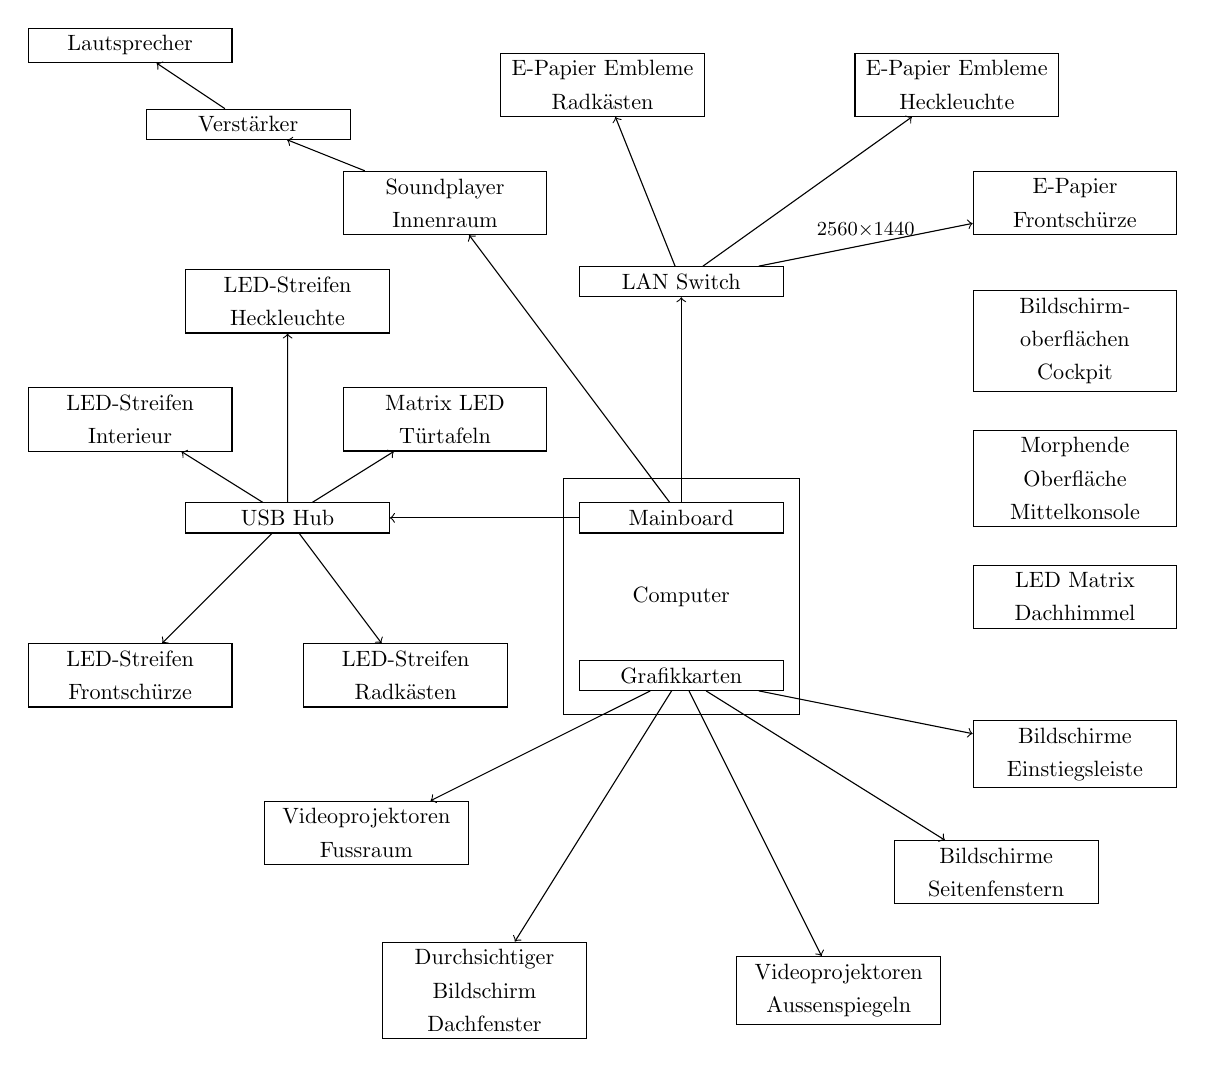
\begin{tikzpicture}[every node/.style={scale=0.8}]
	\node[text width=3.2cm, align=center] (Computer) at (0, -1) {Computer};
	\draw[draw=black] (-1.5,-2.5) rectangle ++(3,3);
	\node[draw, rectangle, text width=3cm, align=center] (Mainboard) at (0, 0) {Mainboard};
	\node[draw, rectangle, text width=3cm, align=center] (Grafikkarten) at (0, -2) {Grafikkarten};
	\node[draw, rectangle, text width=3cm, align=center] (LAN Switch) at (0, 3) {LAN Switch};
	\node[draw, rectangle, text width=3cm, align=center] (E-Papier Frontschürze) at (5, 4) {E-Papier Frontschürze};
	\node[draw, rectangle, text width=3cm, align=center] (LED-Streifen Frontschürze) at (-7, -2) {LED-Streifen Frontschürze};
	\node[draw, rectangle, text width=3cm, align=center] (E-Papier Embleme Radkästen) at (-1, 5.5) {E-Papier Embleme Radkästen};
	\node[draw, rectangle, text width=3cm, align=center] (LED-Streifen Radkästen) at (-3.5, -2) {LED-Streifen Radkästen};
	\node[draw, rectangle, text width=3cm, align=center] (Videoprojektoren Aussenspiegeln) at (2, -6) {Videoprojektoren Aussenspiegeln};
	\node[draw, rectangle, text width=3cm, align=center] (Bildschirme Seitenfenstern) at (4, -4.5) {Bildschirme Seitenfenstern};
	\node[draw, rectangle, text width=3cm, align=center] (LED-Streifen Heckleuchte) at (-5, 2.75) {LED-Streifen Heckleuchte};
	\node[draw, rectangle, text width=3cm, align=center] (E-Papier Embleme Heckleuchte) at (3.5, 5.5) {E-Papier Embleme Heckleuchte};
	\node[draw, rectangle, text width=3cm, align=center] (LED-Streifen Interieur) at (-7, 1.25) {LED-Streifen Interieur};
	\node[draw, rectangle, text width=3cm, align=center] (Matrix LED Türtafeln) at (-3, 1.25) {Matrix LED Türtafeln};
	\node[draw, rectangle, text width=3cm, align=center] (Bildschirme Einstiegsleiste) at (5, -3) {Bildschirme Einstiegsleiste};
	\node[draw, rectangle, text width=3cm, align=center] (Videoprojektoren Fussraum) at (-4, -4) {Videoprojektoren Fussraum};
	\node[draw, rectangle, text width=3cm, align=center] (Morphende Oberfläche Mittelkonsole) at (5, 0.5) {Morphende Oberfläche Mittelkonsole};
	\node[draw, rectangle, text width=3cm, align=center] (Durchsichtiger Bildschirm Dachfenster) at (-2.5, -6) {Durchsichtiger Bildschirm Dachfenster};
	\node[draw, rectangle, text width=3cm, align=center] (LED Matrix Dachhimmel) at (5, -1) {LED Matrix Dachhimmel};
	\node[draw, rectangle, text width=3cm, align=center] (Bildschirmoberflächen Cockpit) at (5, 2.25) {Bildschirm-oberflächen Cockpit};
	\node[draw, rectangle, text width=3cm, align=center] (Soundplayer Innenraum) at (-3, 4) {Soundplayer Innenraum};
	\node[draw, rectangle, text width=3cm, align=center] (USB Hub) at (-5, 0) {USB Hub};
	\node[draw, rectangle, text width=3cm, align=center] (Verstärker) at (-5.5, 5) {Verstärker};
	\node[draw, rectangle, text width=3cm, align=center] (Lautsprecher) at (-7, 6) {Lautsprecher};
	\draw[->] (Mainboard) -> (LAN Switch);
	\draw[->] (Mainboard) -> (Soundplayer Innenraum);
	\draw[->] (Mainboard) -> (USB Hub);
	\draw[->] (Grafikkarten) -> (Bildschirme Seitenfenstern);
	\draw[->] (Grafikkarten) -> (Bildschirme Einstiegsleiste);
	\draw[->] (Grafikkarten) -> (Videoprojektoren Fussraum);
	\draw[->] (Grafikkarten) -> (Videoprojektoren Aussenspiegeln);
	\draw[->] (Grafikkarten) -> (Durchsichtiger Bildschirm Dachfenster);
	\draw[->] (LAN Switch) -> node[above]{\small2560$ \times $1440} (E-Papier Frontschürze);
	\draw[->] (LAN Switch) -> (E-Papier Embleme Radkästen);
	\draw[->] (LAN Switch) -> (E-Papier Embleme Heckleuchte);
	\draw[->] (USB Hub) -> (LED-Streifen Frontschürze);
	\draw[->] (USB Hub) -> (LED-Streifen Radkästen);
	\draw[->] (USB Hub) -> (LED-Streifen Heckleuchte);
	\draw[->] (USB Hub) -> (LED-Streifen Interieur);
	\draw[->] (USB Hub) -> (Matrix LED Türtafeln);
	\draw[->] (Soundplayer Innenraum) -> (Verstärker);
	\draw[->] (Verstärker) -> (Lautsprecher);
\end{tikzpicture}
	\caption[Ansteuerung Komponenten im Prototypen]{Ansteuerung Komponenten im Prototypen}
	\label{fig:tikz_ansteuerung}
\end{figure}
\chapter{Analyse der Komponenten des Prototypen}
\label{cha:Analyse}
Nachfolgend werden alle Komponenten unter den von \ref{cha:Kriterien} genannten Kriterien analysiert. Im Zuge der Analyse werden im nächsten Kapitel Entwürfe für die Weiterentwicklung der Komponenten dargestellt.\\
Die Analyse basiert auf den Komponenten des Prototypen, aber beschränkt sich nicht auf die einzeln verbaute Technologie, sondern geht auf den Gesamtkontext der Komponente ein. Grundlegend richtet sich die Analyse nach dem sinnlichen Darstellungszweck und dessen Bedarf an technischen Eigenschaften. \\
Ein Beispiel dieser Herangehensweise ist der Bildschirm in der Einstiegsleiste. Die genaue Größe einer möglichen Serienimplementierung muss nicht gleich des Prototypen sein, aber sie muss eine Größe haben, die für die Darstellung der Inhalte geeignet ist.\\
Die Kriterien für den Einbau und die spätere Analyse basieren zum Einen auf einer selbstständigen Recherche über die Komponenten und den relevanten Bedingungen. Zum Anderen wurden Informationen von Experten in den einzelnen Fachgebieten der Karosserieinnenentwicklung, Individualisierung, After-Sales-Produktentwicklung herangezogen, um die Kriterien im Bereich rechtlich, wirtschaftlich und technische anzuwenden. \\
Für einen Überblick über die Erkenntnisse fasst das Unterkapitel \ref{ZusammendassungAnalyse} die Analyse zusammen.
\section{Kriterien für den Einbau der Komponenten in Serienfahrzeuge}
\label{cha:Kriterien}
Die folgenden Kriterien richten sich zum einen an die Komponenten und zum anderen an die Fahrzeugentwicklung. Anhand der Kriterien kann eine Analyse des Ist-Zustandes durchgeführt werden.\\
Da für den Verkauf und Betrieb von Fahrzeugen die gültigen Gesetze und Normen eingehalten werden müssen, haben die rechtlichen Kriterien die oberste Priorität. Wenn alle rechtlichen Bedingungen erfüllt sind, stellen sich betriebswirtschaftliche Fragestellungen, ob die Komponenten in Ihrer Funktion einen Nutzen für den Kunden und für das Unternehmen haben. Dies können hier besonders auch optische Vorteile sein. Zuletzt müssen technische Kriterien von der Seite der Fahrzeugentwicklung und der Komponenten erfüllt sein, damit die Weiterentwicklung der Komponenten in Erwägung gezogen werden kann. \\
Durch den zeitlichen Rahmen dieser Arbeit und dem fachlichen Schwerpunkt in elektrotechnischen Systemen, liegt der Fokus der Analyse in der technischen Analyse des Strombedarfs und des Informationsbedarfs. Dennoch soll diese Arbeit die wichtigsten Aspekte und eine Einordnung der anderen Fachbereiche liefern.\\
Nachfolgend werden mit der gleichen Reihenfolge wie oben die Kriterien definiert.
\subsection{Rechtliche Kriterien}
Unter rechtlichen Kriterien finden sich alle Bedingungen für die Fahrzeugentwicklung, die auf Basis von Gesetzen und Normen für eine Zulassung erfüllt werden müssen. Diese Kriterien gewährleisten zugleich Rechtssicherheit für den Hersteller. \\
Aus Gründen des Überblicks wird in der folgenden Arbeit nur auf einzelne Themen von rechtlichen Kriterien eingegangen. 
Ein Beispiel für rechtliche Kriterien ist die europäische Richtlinie ECE R48 für Lichter am Fahrzeug. \cite[Vgl. Seite 1 ff.]{R48.2016} \\
Im Rahmen einer weiteren Entwicklung von Komponenten für eine Fahrzeugserie sind die rechtlichen Bedingungen unbedingt frühzeitig von internen oder externen Juristen und Juristinnen zu prüfen.
\subsection{Wirtschaftliche Kriterien}
Unter wirtschaftliche Kriterien fallen sowohl betriebswirtschaftliche Betrachtungen als auch kundenspezifische Anforderungen. Diese Aspekte sind Grundvoraussetzungen für eine Erstellung eines positiven Geschäftsplan und sollen somit einen Rahmen in diesem Bereich bieten. Die weiteren Schritte nach Erfüllung dieser Kriterien sind Absprachen mit Produktstrategen, Marketingexperten und Kalkulatoren. \\
Unter dem betriebswirtschaftlichen Kriterium steht in erster Linie die Gewinnerzielungsabsicht, das heißt die Kosten des Produkts sollen geringer als die möglichen Einnahmen sein. Kosten können neben den Entwicklungskosten und Produktionskosten für die Komponente, auch Verwaltungskosten über den Lebenszyklus des Produkts und Anpassungskosten anderer Bauteile im Fahrzeug sein. \\
Einnahmen sind neben dem Verkauf der Komponente als Sonderausstattung weitere sekundäre Möglichkeiten durch digitale Produkte spezifisch zu den Komponenten. Daneben können es auch nicht monetäre Einnahmen geben, die das gesamte Produkt und die Marke in ihrem Ansehen stärken.\\
Um einen Gewinn zu erwirtschaften, muss die Komponente mit ihren Fixkosten, wie die Entwicklung, und ihren variablen Kosten, wie den Produktionskosten, gering sein, aber dennoch einen großen Mehrwert für den Kunden liefern, damit die Nachfrage an der Komponente steigt. \\
Die Entwicklungskosten sind abhängig vom aktuellen Reifegrad vorhandener Technik und der Komplexität der Technik, während Anpassungskosten abhängig sind von dem entstehenden Bedarf an Architekturveränderungen. Die Produktionskosten sind abhängig von den Einkaufspreisen der Komponenten und der Montage. \\
Auf der Seite der Einnahmen steht im Mittelpunkt das Kundeninteresse für den Kauf solcher Komponenten. Kriterien für den Kauf von Komponenten durch Kunden können durch Probandenstudien gewonnen werden oder aus Erfahrung von ähnlichen Projekten herangezogen werden. \\
Diese wirtschaftlichen Kriterien werden in dieser Arbeit nach der technischen Analyse gesammelt betrachtet. Das Gesamtkonzept für das Fahrzeug fordert eine ganzheitliche Inszenierung des Fahrzeugs, wofür mehrere Komponenten benötigt werden, um diesen Effekt zu erzielen. Aus diesem Hintergrund ist es sinnvoll die Entwicklung der Komponenten ganzheitlich wirtschaftlich zu bewerten. \\
\subsection{Technische Kriterien}
Unter technischen Kriterien fallen alle relevanten Gebiete für eine erste Untersuchung für die Produktentwicklung:
\begin{enumerate}
	\item Physikalische Dimensionierung
	\item Stabilität
	\item Gewicht
	\item Elektrischer Energiebedarf
	\item Informationsbedarf
	\item Optik
	\item Wartungsfähigkeit
\end{enumerate}
Je nach Beschaffenheit der Komponenten können diese Gebiete unterschiedlich ins Gewicht fallen.
\paragraph{Physikalische Dimensionierung}
Zur erfolgreichen Integration der Komponente in ein Fahrzeug muss an der gewünschten Stelle genügend Bauraum zur Verfügung stehen.
\paragraph{Stabilität}
Die Komponente muss an der Einbaustelle befestigt werden können. Alle Stabilität- und Crashtests müssen positiv ausfallen.
\paragraph{Gewicht}
Das Fahrzeug muss das zusätzliche Gewicht der Komponenten an dieser Stelle aufnehmen können.
\paragraph{Elektrischer Energiebedarf}
Die Komponente soll einen möglichst geringen Strombedarf haben, während das Fahrzeug diesen an der Stelle zur Verfügung stellen muss.
\paragraph{Informationsbedarf}
Zur Steuerung der Komponente muss an der Stelle eine Möglichkeit vorhanden sein, mit dem Gesamtfahrzeug zu kommunizieren. Kriterien sind zum einen die benötigte Bandbreite der Komponenten und die Geschwindigkeit des Informationsaustausches. \\
In der folgenden Arbeit wird bei Videos mit einer Frame-Rate von 24 Bilder pro Sekunde ausgegangen und einer Farbtiefe pro Farbe von einem Byte. Bei Bildern wird ein Kompressionsfaktor von zehn genutzt. Wie bei \ref{cha:Prototyp} erwähnt, sollen zehn Kollektionen mit fünf Inhalten im System gespeichert sein und in Echtzeit aufgerufen werden können. Ein Inhalt kann ein Bild oder ein Video mit einer Länge von zehn Sekunden sein.
Die Berechnung des Speicherbedarfes dient als erste Abschätzung für die Speicherdimensionierung und kann vom tatsächlichen Bedarf abweichen, da die Rechnung Prüf- und Steuerdaten nicht beachtet.
\paragraph{Optische Kriterien}
Unter optischen Kriterien fallen alle allgemein gültige Designprinzipien in der Produktentstehung. Darunter versteht sich die Harmonie der Komponenten in der Umgebung, die Vermeidung von Bildschirmrändern, usw.
\paragraph{Wartungsfähigkeit}
Unter Wartungsfähigkeit fällt der leichte Ein- und Ausbau der Komponente bei Bedarf und der Austausch von Verschleißgegenständen.
\section{Analyse der Exterieur Komponenten}
Im folgenden werden die Exterieur Komponenten an Hand der oben beschriebenen einzelnen Kriterien geprüft. Die wirtschaftlichen Kriterien werden in einem separaten Abschnitt gesammelt betrachtet. 
\subsection{E-Papier in der Frontschürze}
Rechtlich ist zu Prüfen, ob das E-Papier als Leuchte gilt und danach behandelt werden muss. Daneben sind die rechtlichen Grundlagen für das Ändern der Bildschirminhalten in unterschiedlichen Fahrmodi, wie zum Beispiel Parken oder Fahren, zu analysieren. \\
Wirtschaftlich betrachtet ist diese Komponente ein zentraler Bestandteil des Fahrzeugkonzeptes, da durch die Größe und Lage der Kunde die Inhalte stark wahrnimmt. \\
Mit einer physikalischen Dimensionierung über die gesamte Breite zwischen den Frontlichtscheinwerfern und somit eine mögliche Breite bei unterschiedlichen Fahrzeugmodellen von 80 cm bis 1 m und einer Höhe von 50 cm bis 60 cm ist die Stabilität des E-Papiers zu prüfen, da die Lage im Kotflügel besonders transponiert ist. \\ 
Das zusätzliche Gewicht des Bildschirms ist an der vorderen Kotflügelbefestigung aufzunehmen.\\
Der Strombedarf des E-Papier ist, wie in \ref{cha:Grundlagen} beschrieben, nur gering. Ein Mikrocontroller zur Steuerung benötigt zum Beispiel eine Spannung von 12V Gleichstrom. \\
Mit einer Auflösung von 2560 Pixel pro Zeile zu 1440 Zeilen und einer Farbtiefe von 16 Stufen benötigt das Display mit der Formel \ref{eq:Bilddatenmenge} pro Bild einen Speicher S von $ 368,64\,\mathrm{kByte} $. 
\begin{align}
	S &= \frac{2560\,\frac{\mathrm{Pixel}}{\mathrm{Zeile}}\times 1440\,\mathrm{Zeilen} \times 8\,\frac{\mathrm{Bit}}{\mathrm{Pixel}}}{10} \\
	&=  368,64\,\mathrm{kByte}
\end{align}
Bei zehn Kollektionen mit jeweils fünf Bildern benötigt man einen Speicher von $ 18,432\,\mathrm{MByte} $. \\
Durch die Position ist die gezielte Brechung bei Crashs relevant für die Sicherheit von Passanten.
Daneben ist zu Prüfen, ob die Radarsensorik von dem E-Papier gestört wird.\\
\subsection{LED-Streifen in der Frontschürze}
Unter den rechtlichen Kriterien gilt bei Lichtern die europäische Richtlinie ECE R48. Farbliche Lichter außerhalb der zulässigen Verbauten sind dabei nicht gestattet. Daher gilt es zu prüfen, welche weitere Möglichkeiten dieser Darstellungsart es gibt. Optionen sind beispielsweise schwarz-weiße Lichter oder farbliche Bildschirme ohne aktive Beleuchtung. \\
Für eine Farbtiefe von 256 Stufen pro Farbe benötigt jede einzelne LED 24 Bit an Speicher, da es drei mal acht Bit benötigt. Bei 332 LEDs bedeutet das einen Speicher pro Bild von $ 996\,\mathrm{Byte} $.
\begin{align}
	S &= \frac{332\,\mathrm{Pixel} \times 24\,\frac{\mathrm{Bit}}{\mathrm{Pixel}}}{1} \cdot \\
	&=  996\,\mathrm{Byte}
\end{align}
Für ein 10 Sekunden Video wird ein Speicher S von 
\begin{align}
	S &= 996\,\mathrm{Byte} \cdot 24\,\mathrm{fps} \cdot 10\,\mathrm{s}\\
	&= 239,04\,\mathrm{kByte}
\end{align}
benötigt. Bei insgesamt 50 Inhalten bedeutet das $ 11,952\,\mathrm{MByte} $ an Speicherbedarf. \\
Eine farbige LED, die pro Pixel vier Dioden (Rot, Grün, Blau und Weiß) enthält, hat einen Leistungsaufnahme von $ 320\,\mathrm{mW} $.  
Die LED-Streifen benötigen mit einer Anzahl von 500 LED eine Leistung von $ 160\,\mathrm{W} $. Im 12 V Bordnetz beträgt die Stromstärke $ 13,3\,\mathrm{A} $. 
Daneben muss eine Ansteuerungslogik dort verbaut werden.
\subsection{E-Papier Embleme über den vorderen Radkästen}
Die E-Papiere an den Fahrzeugseiten müssen, wie oben erwähnt, geprüft werden, ob sie als Beleuchtung gelten.\\
Aus Sicht der Kunden ist die Lage neben den Fronttüren ideal, um Dinge anzuzeigen.
Da auf diesen E-Papieren vorwiegend Text angezeigt wird, ist ein breites und in der Höhe schmales Display von Vorteil, da dort eine Zeile leserlich angezeigt werden kann. \\
Um bei Beschädigung oder bei Defekt das E-Papier auszutauschen, ist die Möglichkeit über den Zugriff vom Motorraum aus zu prüfen. \\
Das Gewicht des E-Papiers ist relativ gering und zu vernachlässigen.
Da das E-Papier nur bei Änderung des Inhaltes Strom verbraucht, muss nur eine geringe Leistungsaufnahme von $ x\,\mathrm{mW} $ sichergestellt werden. \\
Die E-Papier Embleme benötigen mit einer Auflösung von 1600 Pixel pro Zeile zu 1200 Zeilen einen Speicher pro Bild von $ 192\,\mathrm{kByte} $.
\begin{align}
	S &= \frac{1600\,\frac{\mathrm{Pixel}}{\mathrm{Zeile}} \times 1200\,\mathrm{Zeilen} \times 8\,\frac{\mathrm{Bit}}{\mathrm{Pixel}}}{10} \cdot \\
	&= 192\,\mathrm{kByte}
\end{align}
Insgesamt benötigt der Speicher eine Größe von $ 9,6\,\mathrm{MByte} $ für 50 Bilder.
\subsection{LED-Streifen in den Radkästen}
Wie bei den anderen Leuchteinrichtungen im Exterieur sind hier die Marktregularien zu prüfen. Bei Möglichkeit kann auch ein eingeschränkter Modus von schwarz-weißem Licht oder nur die Anzeige im abgestellten Zustand des Fahrzeuges gewählt werden. \\
Die Verschmutzung des Lichtleiters ist durch eine geeignete Konstruktion zu verhindern und daneben auch der Beschädigung durch geschleuderte Steine oder ähnliches. \\
Daneben muss aus Kundensicht geprüft werden, ob die Betonung des Schmutzfänger Bereichs gewünscht ist, oder nur in bestimmten Situationen.
Bei einer Anzahl von 200 LED pro Radkasten benötigt ein LED Streifen eine Leistung von $ 64\,\mathrm{W} $.
Ein dynamisches Lichtspiel für 10 Sekunden benötigt pro Radkasten bei einer Bildwiederholungsrate von $ 24\,\mathrm{fps} $ einen Speicher von $ 144\,\mathrm{kByte}$. \\
\begin{align}
	S &= \frac{200\,\mathrm{Pixel} \times 24\,\frac{\mathrm{Bit}}{\mathrm{Pixel}}}{1} \cdot \\
	&= 600\,\mathrm{Byte}
\end{align}
\begin{align}
	S &= 600\,\mathrm{Byte} \cdot 24\,\mathrm{fps} \cdot 10\,\mathrm{s}\\
	&= 144\,\mathrm{kByte}
\end{align}
Für 50 Videos beträgt die Speichergröße $ 7,2\,\mathrm{MByte} $.
Die Vernetzung an dieser Stelle ist eine Herausforderung.
\subsection{Videoprojektoren in den Außenspiegeln}
Die Verfügbarkeit des Bauraums in dem Außenspiegel ist zu prüfen, indem der Bauraum von aktuellen Standbildprojektoren mit den benötigten Videoprojektoren verglichen wird. 
Daneben ist die Zulässigkeit von solchen Projektionen und deren Lichtaustrittsfläche rechtlich abzuprüfen. \\
Die angestrahlte Fläche auf dem Boden reicht im besten Fall über die gesamten Seitentüren und bis zu $ 2\,\mathrm{m} $ weg vom Fahrzeug.
Der Betrachter soll bei unterschiedlichen Lichtverhältnissen noch ein möglichst kontrastreiches und helles Bild erkennen. \\
Der Strombedarf pro Videoprojektor liegt im Bereich zwischen $ XX\,\mathrm{W} $ und $ XX\,\mathrm{W} $.
Ein Standbild benötigt bei einer Pixelanzahl pro Zeile von $ 1280 $ und $ 800 $ Zeilen ein Speichergröße von ca. $ 256\,\mathrm{kByte}$. 
\begin{align}
	S &= \frac{1280\,\frac{\mathrm{Pixel}}{\mathrm{Zeile}} \times 800\,\mathrm{Zeilen} \times 24\,\frac{\mathrm{Bit}}{\mathrm{Pixel}}}{10} \\
	&= 307,2\,\mathrm{kByte}
\end{align}
Für eine Animation von zehn Sekunden Länge benötigt eine Videoprojektor einen Speicher von $ 73,728\,\mathrm{MByte}$.
\begin{align}
	S &= 307,2\,\mathrm{kByte} \cdot 24\,\mathrm{fps} \cdot 10\,\mathrm{s}\\
	&= 73,728\,\mathrm{MByte} 
\end{align}
Insgesamt wird ein Speicher in Höhe von $ 3,6864\,\mathrm{GByte} $ benötigt.
\subsection{Bildschirme in den hinteren Seitenfenstern}
Rechtlich ist die Zulässigkeit wegen möglicher Ablenkungen von Straßenverkehrsteilnehmern zu prüfen.
Das Verkleinern der Fensterfläche ist abzuprüfen, ob dies mit Kundeninteressen vereinbar ist.
Die Crashsicherheit an dieser Stelle und die Stabilität ist wichtig, da sich diese Komponente. in unmittelbarer Nähe zu den Fahrzeuginsassen befindet.
Jedes Display hat eine ungefähre Leistung von $ XX\,\mathrm{W} $. 
Ein Standbild benötigt bei einer Pixelanzahl pro Zeile von $ 1280 $ und von $ 800 $ Zeilen ein Speichergröße von ca. $ 307,2\,\mathrm{kByte}$. 
\begin{align}
	S &= \frac{1280\,\frac{\mathrm{Pixel}}{\mathrm{Zeile}}\times 800\,\mathrm{Zeilen} \times 24\,\frac{\mathrm{Bit}}{\mathrm{Pixel}}}{10} \\
	&= 307,2\,\mathrm{KByte}
\end{align}
Für eine Animation von zehn Sekunden Länge benötigt das Display einen Speicher von $ 73,728\,\mathrm{MByte}$.
\begin{align}
	S &= 307,2\,\mathrm{kByte} \cdot 24\,\mathrm{fps} \cdot 10\,\mathrm{s}\\
	&= 73,728\,\mathrm{MByte}
\end{align}
Insgesamt wird ein Speicher pro Bildschirm von $ 3,6864\,\mathrm{GByte} $ benötigt.
\subsection{LED-Streifen in der Heckleuchte}
Wie bei den LED-Streifen in der Frontschürze sind die rechtlichen und wirtschaftlichen Fragestellungen gleich. \\
Grundsätzlich gilt es zu prüfen, ob die vorhandenen Steuergeräte für die Lichter Kapazitäten für dynamische Lichtstreifen frei haben.
Die weiteren technischen Kriterien verhalten sich wie oben erläutert. \\
Für ein Bild benötigt man einen Speicher von $ 1,173\,\mathrm{kByte} $.
\begin{align}
	S &= \frac{391\,\mathrm{Pixel} \times 24\,\frac{\mathrm{Bit}}{\mathrm{Pixel}}}{1} \cdot \\
	&= 1,173\,\mathrm{kByte}
\end{align}
Für eine zehn Sekunden Inszenierung sind $ 281,52\,\mathrm{kByte} $ erforderlich.
\begin{align}
	S &= 1,173\,\mathrm{kByte} \cdot 24\,\mathrm{fps} \cdot 10\,\mathrm{s} \\
	&= 281,52\,\mathrm{kByte}
\end{align}
Insgesamt wird ein Speicher von $ 14,076\,\mathrm{MByte} $ benötigt.
\subsection{E-Papier in der Heckleuchte}
Ähnliche Anforderungen wie die E-Papier Embleme über den vorderen Radkästen haben diese E-Papiere in der Heckleuchte
Diese E-Papiere in der Heckleuchte haben ähnliche Eigenschaften, wie die E-Papier Embleme über den vorderen Seitenkästen, in Bezug auf die rechtlichen Kriterien. Durch die Position in der Nähe der Heckleuchten kann von dort die Stromversorgung und Busanbindung bezogen werden. Der Strombedarf und Datenspeicherbedarf von $ 160\,\mathrm{kByte} $ pro Bild sind gleich mit dem anderen E-Papier. 
\begin{align}
	S &= \frac{1600\,\mathrm{Pixel pro Zeile} \times 1200\,\mathrm{Zeilen} \times 8\,\frac{\mathrm{Bit}}{\mathrm{Pixel}}}{10} \cdot \\
	&= 192\,\mathrm{kByte}
\end{align}
Für 50 Bilder sind es dementsprechend $ 9,6\,\mathrm{MByte} $.
\section{Analyse der Interieur Komponenten}
Im folgenden werden die einzelnen Interieur Komponenten mit den Kriterien analysiert.
\subsection{LED-Streifen im Interieur}
Rechtlich ist bei den Animationen im LED-Streifen die Vermeidung von Ablenkung des Fahrers oder der Fahrerin zu gewährleisten.
Durch die Länge des Streifens muss für die Crashsicherheit eventuelle Sollbruchstellen sichergestellt werden. \\
Bei einer Anzahl von 719 LED pro Radkasten benötigt ein LED Streifen eine Leistung von $ XX\,\mathrm{W} $.
Für eine Inszenierung von zehn Sekunden Länge benötigt der LED-Streifen Speicherplatz in der Höhe von $ 25,884\,\mathrm{MByte}$.
\begin{align}
	S &= \frac{719\,\mathrm{Pixel} \times 24\,\frac{\mathrm{Bit}}{\mathrm{Pixel}}}{1} \cdot \\
	&= 2,157\,\mathrm{kByte}
\end{align}
\begin{align}
	S &= 2,157\,\mathrm{kByte} \cdot 24\,\mathrm{fps} \cdot 10\,\mathrm{s}\\
	&= 517,68\,\mathrm{kByte}
\end{align}
Für 50 Videos beträgt die Speichergröße $ 25,884\,\mathrm{MByte} $.
\subsection{LED Türtafeln}
Rechtlich gesehen ist zu prüfen, ab welchem Helligkeitsgrad und Farbinszenierung der Fahrer oder die Fahrerin durch die LED zu stark abgelenkt werden. \\
Im Moment wird nur eine LED pro Türtafel genutzt, wodurch Möglichkeiten der Inszenierung im Vergleich zu einer LED-Matrix nicht genutzt werden. 
Die LEDs benötigen eine Leistung von $ XX\,\mathrm{W} $ pro Türe.
Die Ansteuerung der Türtafeln kann durch die Nähe zu den LED-Streifen im Interieur zusammen gesteuert werden.
\subsection{Bildschirme in der Einstiegsleiste}
Unter den rechtlichen Aspekten gibt es in einer ersten Untersuchung keine Beschränkungen, da der Bildschirm nur bei geöffneter Türe und dementsprechend im Stand betrachtet werden kann.
Die technische Umsetzbarkeit ist durch Bestätigung in ersten Voruntersuchungen (wie Kugelfalltest, Bauraum, Shaker) positiv.
Technische Herausforderungen an dieser Stelle sind Feuchtigkeitsschutz, Temperaturempfindlichkeit, und die Kratzfestigkeit. \\
Jedes Display hat eine ungefähre Leistung von $ XX\,\mathrm{W} $. 
Ein Standbild benötigt bei einer Pixelanzahl pro Zeile von $ 1280 $ und von $ 1024 $ Zeilen ein Speichergröße von ca. $ 393,216\,\mathrm{kByte}$. 
\begin{align}
	S &= \frac{1280\,\frac{\mathrm{Pixel}}{\mathrm{Zeile}}\times 1024\,\mathrm{Zeilen} \times 24\,\frac{\mathrm{Bit}}{\mathrm{Pixel}}}{10} \\
	&= 393,216\,\mathrm{KByte}
\end{align}
Für eine Animation von zehn Sekunden Länge benötigt das Display einen Speicher von $ 94,37184\,\mathrm{MByte}$.
Insgesamt bei 50 Videos beträgt der benötigte Speicher $ 4,718592\,\mathrm{GByte}$.
\subsection{Videoprojektoren im Fußraum}
Unter den rechtlichen Fragestellungen ergibt sich die Vermeidung von Ablenkung für den Fahrer oder die Fahrerin.
Aus Kundenperspektive ist die angestrahlte Oberfläche eventuell nicht geeignet, da diese stärker verschmutzt sein kann. \\
Unter den technischen Kriterien ist die Verfügbarkeit des Bauraums mit der benötigten Kühlung zu prüfen. Eine Herausforderung ist die Befestigung des Videoprojektors, da dieser sich bei Fahrt relativ zum Auto nicht bewegen darf.
Jeder Videoprojektor hat eine ungefähre Leistung von $ XX\,\mathrm{W} $. 
Ein Standbild benötigt bei einer Pixelanzahl pro Zeile von $ 1280 $ und von $ 800 $ Zeilen ein Speichergröße von ca. $ 307,2\,\mathrm{kByte}$. 
\begin{align}
	S &= \frac{1280\,\frac{\mathrm{Pixel}}{\mathrm{Zeile}}\times 800\,\mathrm{Zeilen} \times 24\,\frac{\mathrm{Bit}}{\mathrm{Pixel}}}{10} \\
	&= 307,2\,\mathrm{kByte}
\end{align}
Für eine Animation von zehn Sekunden Länge benötigt das Display einen Speicher von $ 73,728\,\mathrm{MByte}$.
Insgesamt bei 50 Videos beträgt der benötigte Speicher $ 3,6864\,\mathrm{GByte}$.
\subsection{Morphende Oberfläche in der Mittelkonsole}
Die tatsächlich verwendete technische Realisierung der morphenden Oberfläche ist eine Übergangslösung für eine neue Technik, die einzelne Element auf einer Fläche gesteuert hoch und herunterfahren kann. Diese Technik ist derzeit in der Entwicklung. Wie die Farbtiefe bei einem Bildschirm kann die Höhe der einzelnen Punkte eingestellt werden. \\
Mit 8 Bit Höhentiefe benötigt ein Feld mit 20 auf 20 einzelnen Punkten einen Speicher in der Größe von $ 400\,\mathrm{Byte}$.
Eine weitere technische Weiterentwicklung kann Animationen auf der Mittelkonsole abspielen. Die Datenmenge steigert sich dementsprechend mit der Bildwiederholungsrate und der Dauer der Animation. Bei einer Bildwiederholungsrate von $ 24\,\mathrm{fps} $ und 10 Sekunden Dauer beträgt der benötigte Speicher $ 96\,\mathrm{kByte}$.
\subsection{Durchsichtiger Bildschirm im Dachfenster}
Rechtlich betrachtet ist die 
Technische Herausforderungen sind die Temperaturentwicklung durch Sonneneinstrahlung und die Kontaktierung bei Bewegung des Glasdaches.
Das Display hat eine ungefähre Leistung von $ XX\,\mathrm{W} $. 
Ein Standbild benötigt bei einer Pixelanzahl pro Zeile von $ 1920 $ und von $ 1080 $ Zeilen ein Speichergröße von ca. $ 207,36\,\mathrm{kByte}$. 
\begin{align}
	S &= \frac{1920\,\frac{\mathrm{Pixel}}{\mathrm{Zeile}}\times 1080\,\mathrm{Zeilen} \times 8\,\frac{\mathrm{Bit}}{\mathrm{Pixel}}}{10} \\
	&= 207,36\,\mathrm{kByte}
\end{align}
Für eine Animation von zehn Sekunden Länge benötigt das Display einen Speicher von $ 49,7664\,\mathrm{MByte}$.
Insgesamt bei 50 Videos beträgt der benötigte Speicher $ 2,488320\,\mathrm{GByte}$.
\subsection{LED-Matrix im Dachhimmel}
Die LED-Matrix hat eine ungefähre Leistung von $ XX\,\mathrm{W} $. 
Ein Standbild benötigt bei einer Pixelanzahl pro Zeile von $ 192 $ und von $ 96 $ Zeilen ein Speichergröße von ca. $ 55,296\,\mathrm{kByte}$. 
\begin{align}
	S &= \frac{192\,\frac{\mathrm{Pixel}}{\mathrm{Zeile}}\times 96\,\mathrm{Zeilen} \times 24\,\frac{\mathrm{Bit}}{\mathrm{Pixel}}}{1} \\
	&= 55,296\,\mathrm{kByte}
\end{align}
Für eine Animation von zehn Sekunden Länge benötigt das Display einen Speicher von $ 13,27104\,\mathrm{MByte}$.
Insgesamt bei 50 Videos beträgt der benötigte Speicher $ 663,552\,\mathrm{MByte}$.
\subsection{Duftflakons im Innenraum}
Eine technische Verbreitung unterschiedlicher individueller Düfte ist in diesem Konzept nicht realisiert. Ein aktueller technischer Aufbau besteht aus einem Set mit unterschiedlichen Duftflakons, die einzeln geöffnet werden. Dadurch ist die Anzahl der Düfte beschränkt auf die Set-Größe.
\subsection{Bildschirmoberflächen im Cockpit}
Das Anzeigen individualisierter Bildschirmoberflächen auf vorhandenen Displays ist unter den oben beschrieben Kriterien schon im Fahrzeug möglich und benötigt keine weitere Analyse.
\subsection{Soundplayer im Innenraum}
Das Abspielen individualisierter Sounds durch vorhandene Lautsprecher ist unter den oben beschrieben Kriterien schon im Fahrzeug möglich und benötigt keine weitere Analyse.
\subsection{Zusammenfassung Analyse} \label{ZusammendassungAnalyse}
In der Tabelle \ref{tab:Speicherbedarf} werden die Komponenten, die visuelle oder haptische Anzeigen sind, mit dem benötigten Speicher für die Anzeige eines Bildes dargestellt. Die Berechnung erfolgt mit der Gleichung \ref{eq:Bilddatenmenge}.
\begin{table}[hbt]	
	\centering
	\renewcommand{\arraystretch}{1.5}	% Skaliert die Zeilenhöhe der Tabelle
	\captionabove[Berechnung des Speicherbedarfes für ein Bild]{Berechnung des Speicherbedarfes für ein Bild}
	\label{tab:Speicherbedarf}
	\begin{tabular}{c|cccc}
		\textbf{Komponente} & \parbox[t]{0.1\linewidth}{\centering Pixel} & \parbox[t]{0.11\linewidth}{\centering Bit pro Pixel} & \parbox[t]{0.15\linewidth}{\centering Kompression} & \parbox[t]{0.1\linewidth}{\centering Speicher} \\ 
		\hline 
		\hline 
		\parbox[t]{0.3\linewidth}{\centering E-Papier in der Frontschürze} & $ 2560 \times 1440 $ & $ 8 $ & $ 10 $ & $ 368,64\,\mathrm{kByte} $\\ \parbox[t]{0.3\linewidth}{\centering E-Papier Embleme über\\den vorderen Radkästen} & $ 1600 \times 1200 $ & $ 8 $ & $ 10 $ & $ 192\,\mathrm{kByte} $ \\
		\parbox[t]{0.3\linewidth}{\centering E-Papier in der Heckleuchte} & $ 1600 \times 1200 $ & $ 8 $ & $ 10 $ & $ 192\,\mathrm{kByte} $ \\
		\parbox[t]{0.3\linewidth}{\centering LED-Streifen in der Frontschürze} & $ 332 \times 1 $ & $ 24 $ & $ 1 $ & $ 996\,\mathrm{Byte} $ \\
		\parbox[t]{0.3\linewidth}{\centering LED-Streifen in den Radkästen} & $ 200 \times 1 $ & $ 24 $ & $ 1 $ & $ 600\,\mathrm{Byte} $\\ \parbox[t]{0.3\linewidth}{\centering LED-Streifen in der Heckleuchte} & $ 391 \times 1 $ & $ 24 $ & $ 1 $ & $ 1,173\,\mathrm{kByte} $ \\ 
		\parbox[t]{0.3\linewidth}{\centering LED-Streifen im Interieur} & $ 719 \times 1 $ & $ 24 $ & $ 1 $ & $ 2,157\,\mathrm{kByte} $ \\
		\parbox[t]{0.3\linewidth}{\centering LED Türtafeln} & $ 4 \times 1 $ & $ 24 $ & $ 1 $ &  $ 12\,\mathrm{Byte} $ \\
		\parbox[t]{0.3\linewidth}{\centering Videoprojektoren in\\den Außenspiegeln} & $ 1280 \times 800 $ & $ 24 $ & $ 10 $ &   $ 307,2\,\mathrm{kByte} $ \\ 
		\parbox[t]{0.3\linewidth}{\centering Videoprojektoren im Fußraum} & $ 1280 \times 800 $ & $ 24 $ & $ 10 $ & $ 307,2\,\mathrm{kByte} $ \\
		\parbox[t]{0.3\linewidth}{\centering Bildschirme in den\\hinteren Seitenfenstern} & $ 1280 \times 800 $ & $ 24 $ & $ 10 $ & $ 307,2\,\mathrm{kByte} $ \\
		\parbox[t]{0.3\linewidth}{\centering Bildschirme in der Einstiegsleiste} &  $ 1280 \times 1024 $ & $ 24 $ & $ 10 $ & $ 393,216\,\mathrm{kByte} $ \\
		\parbox[t]{0.3\linewidth}{\centering Durchsichtiger Bildschirm\\im Dachfenster} & $ 1920 \times 1080 $ & $ 8 $ & $ 10 $ & $ 207,36\,\mathrm{kByte} $ \\
		\parbox[t]{0.3\linewidth}{\centering LED-Matrix im Dachhimmel} & $ 192 \times 96 $ & $ 24 $ & $ 1 $ & $ 55,296\,\mathrm{kByte} $ \\
		\parbox[t]{0.3\linewidth}{\centering Morphende Oberfläche\\in der Mittelkonsole} & $ 20 \times 20 $ & $ 8 $ & $ 1 $ & $ 400\,\mathrm{Byte} $ \\
	\end{tabular} 
\end{table}
Die unterschiedlichen Datenmengen zwischen $ 12\,\mathrm{Byte} $ und $ 393,216\,\mathrm{kByte} $ für ein Bild, machen deutlich, dass eine Abwägung zwischen hoher Pixelanzahl und Farbtiefe gemacht werden muss. Die benötigte Speichergröße wird neben dem Leistungsbedarf in der Tabelle \ref{tab:Werte} dargestellt. Es wird deutlich, dass das Anzeigen von bewegt Bildern mehr Daten benötigt.
\begin{table}[hbt]	
	\centering
	\renewcommand{\arraystretch}{1.5}	% Skaliert die Zeilenhöhe der Tabelle
	\captionabove[Liste der Komponenten mit den oben festgestellten Werten]{Liste der Komponenten mit den oben festgestellten Werte}
	\label{tab:Werte}
	\begin{tabular}{c|cc}
		\textbf{Komponente} & \parbox[t]{0.16\linewidth}{\centering Leistungs-\\bedarf} & \parbox[t]{0.16\linewidth}{\centering Speicher-\\größe} \\ 
		\hline 
		\hline 
		\parbox[t]{0.3\linewidth}{\centering E-Papier in der Frontschürze} & $ X\,\mathrm{W} $ & $ 18,432\,\mathrm{MByte} $  \\
		\parbox[t]{0.3\linewidth}{\centering E-Papier Embleme über\\den vorderen Radkästen} & $ X\,\mathrm{W} $ & $ 9,6\,\mathrm{MByte} $ \\
		\parbox[t]{0.3\linewidth}{\centering E-Papier in der Heckleuchte} & $ X\,\mathrm{W} $ & $ 9,6\,\mathrm{MByte} $ \\
		\parbox[t]{0.3\linewidth}{\centering LED-Streifen in der Frontschürze} & $ X\,\mathrm{W} $ & $ 11,952\,\mathrm{MByte} $ \\
		\parbox[t]{0.3\linewidth}{\centering LED-Streifen in den Radkästen} & $ X\,\mathrm{W} $ & $ 7,2\,\mathrm{MByte} $ \\ 
		\parbox[t]{0.3\linewidth}{\centering LED-Streifen in der Heckleuchte} & $ X\,\mathrm{W} $ & $ 14,076\,\mathrm{MByte} $ \\ 
		\parbox[t]{0.3\linewidth}{\centering LED-Streifen im Interieur} & $ X\,\mathrm{W} $ & $ 25,884\,\mathrm{MByte} $ \\
		\parbox[t]{0.3\linewidth}{\centering LED Türtafeln} & $ X\,\mathrm{W} $ & $ 144\,\mathrm{KByte} $ \\
		\parbox[t]{0.3\linewidth}{\centering Videoprojektoren in\\den Außenspiegeln} & $ X\,\mathrm{W} $ & $ 3,6864\,\mathrm{GByte} $ \\ 
		\parbox[t]{0.3\linewidth}{\centering Videoprojektoren im Fußraum} & $ X\,\mathrm{W} $ & $ 3,6864\,\mathrm{GByte} $ \\
		\parbox[t]{0.3\linewidth}{\centering Bildschirme in den\\hinteren Seitenfenstern} &$ X\,\mathrm{W} $ & $ 3,6864\,\mathrm{GByte} $ \\
		\parbox[t]{0.3\linewidth}{\centering Bildschirme in der Einstiegsleiste} & $ X\,\mathrm{W} $ & $ 4,718592\,\mathrm{GByte} $ \\
		\parbox[t]{0.3\linewidth}{\centering Durchsichtiger Bildschirm\\im Dachfenster} & $ X\,\mathrm{W} $ & $ 2,48832\,\mathrm{GByte} $ \\
		\parbox[t]{0.3\linewidth}{\centering LED-Matrix im Dachhimmel} & $ X\,\mathrm{W} $ & $ 663,552\,\mathrm{MByte} $ \\
		\parbox[t]{0.3\linewidth}{\centering Morphende Oberfläche\\in der Mittelkonsole} & $ X\,\mathrm{W} $ & $ 4,8\,\mathrm{MByte} $ \\
	\end{tabular} 
\end{table}
In diesem Abschnitt werden die Komponenten als Gesamtes unter den wirtschaftlichen Kriterien betrachtet, weil die Komponenten nicht als einzelne Sonderausstattung, sondern als Ganzes oder Gebündelt vertrieben werden soll. Daher ist eine Gesamtbetrachtung der wirtschaftlichen Kriterien sinnvoll. \\
In Tabelle \ref{tab:Entwicklung} werden alle Komponenten mit den nötigen Anpassungen in der Serienentwicklung in den bestimmten Bereichen auf Basis der vorherigen technischen Analyse. 
\begin{table}[hbt]	
	\centering
	\renewcommand{\arraystretch}{1.5}	% Skaliert die Zeilenhöhe der Tabelle
	\captionabove[Liste der Komponenten mit den nötigen Eingriffen in die Fahrzeugentwicklung]{Liste der Komponenten mit den nötigen Eingriffen in die Fahrzeugentwicklung}
	\label{tab:Entwicklung}
	\begin{tabular}{c|ccc}
		\textbf{Komponente} & \textbf{Karosserie} & \textbf{E/E Architektur} & \textbf{Software} \\ 
		\hline 
		\hline 
		\parbox[t]{0.4\linewidth}{\centering E-Papier in der Frontschürze} & X & X & X \\
		\parbox[t]{0.4\linewidth}{\centering LED-Streifen in der Frontschürze} & X & X & X \\
		\parbox[t]{0.4\linewidth}{\centering E-Papier Embleme über\\den vorderen Radkästen} & X & X & X \\
		\parbox[t]{0.4\linewidth}{\centering LED-Streifen in den Radkästen} & X & X & X \\
		\parbox[t]{0.4\linewidth}{\centering Videoprojektoren in\\den Außenspiegeln} & X & X & X \\
		\parbox[t]{0.4\linewidth}{\centering Bildschirme in den\\hinteren Seitenfenstern} & X & X & X \\
		\parbox[t]{0.4\linewidth}{\centering LED-Streifen in der Heckleuchte} &  & X & X \\
		\parbox[t]{0.4\linewidth}{\centering E-Papier in der Heckleuchte} & X & X & X \\
		\parbox[t]{0.4\linewidth}{\centering LED-Streifen im Interieur} &  & X & X \\
		\parbox[t]{0.4\linewidth}{\centering LED Türtafeln} &  & X & X \\
		\parbox[t]{0.4\linewidth}{\centering Bildschirme in der Einstiegsleiste} &  & X & X \\
		\parbox[t]{0.4\linewidth}{\centering Videoprojektoren im Fußraum} &  & X & X \\
		\parbox[t]{0.4\linewidth}{\centering Morphende Oberfläche\\in der Mittelkonsole} &  & X & X \\
		\parbox[t]{0.4\linewidth}{\centering Durchsichtiger Bildschirm\\im Dachfenster} &  & X & X \\
		LED-Matrix im Dachhimmel & X & X & X \\
		\parbox[t]{0.4\linewidth}{\centering Bildschirmoberflächen im Cockpit} &  &  & X \\
		\parbox[t]{0.4\linewidth}{\centering Soundplayer im Innenraum} &  & X & X \\
		\parbox[t]{0.4\linewidth}{\centering Duftflakons im Innenraum} &  & X & X \\
	\end{tabular} 
\end{table}
		%Der parbox-Befehl ist erforderlich, damit ein Zeilenumbruch erzeugt werden kann. c-Spalten (zentriert) erlauben nicht automatisch einen Zeilenumpruch. Linksbündig gesetzte p-Spalten erlauben automatisch den Zeilenumbruch.%


\chapter{Konzeptentwurf}
\label{cha:Konzeptentwurf}

... Text Konzeptentwurf: Gegenüberstellung verschiedener Lösungsansätze und Lösungsgenerierung, etc.
\chapter{Verifikation und Diskussion}
\label{cha:Verifikation}

... Verifikation, Auswertung, Lösungsbewertung, Diskussion der Ergebnisse


\chapter{Zusammenfassung}
\label{cha:zusammenfassung}

... Text Zusammenfassung und Ausblick: In der Zusammenfassung unbedingt klare Aussagen zum Ergebnis der Arbeit nennen, im Optimalfall quantitative Angaben. Die Inhalte müssen sich auf die Fragestellung aus der Einleitung  beziehen. ...


% ---- Literaturverzeichnis ----------
\interlinepenalty 10000					% Verhindert einen Umbruch mitten in Literatureinträgen
\printbibliography						% Erstellen des Literaturverzeichnisses

% -----Ausgabe aller Verzeichnisse ---
\setlength{\parskip}{0.5\baselineskip}
\renewcommand{\indexname}{Sachwortverzeichnis}
\printindex								% Erzeugen des Indexverzeichnises
\addcontentsline{toc}{chapter}{\indexname}
% alle Abkürzungen, die in der Arbeit verwendet werden. Die Alphabetische Sortierung übernimmt Latex. Nachfolgend sind Beispiele genannt, welche nach Bedarf angepasst, gelöscht oder ergänzt werden können.

% Bei den unten stehenden Formelzeichen ist erläutert, wie explizite Sortierschlüssel über den Inhalt der eckigen Klammer angegeben werden.

% Allgemeine Abkürzungen %%%%%%%%%%%%%%%%%%%%%%%%%%%%
%\nomenclature{Abb.}{Abbildung}
%\nomenclature{bzw.}{beziehungsweise}
%\nomenclature{DHBW}{Duale Hochschule Baden-Württemberg}
%\nomenclature{ebd.}{ebenda}
%\nomenclature{et al.}{at alii}
%\nomenclature{etc.}{et cetera}
%\nomenclature{evtl.}{eventuell}
\nomenclature{f.}{folgende Seite}
\nomenclature{ff.}{fortfolgende Seiten}
%\nomenclature{ggf.}{gegebenenfalls}
%\nomenclature{Hrsg.}{Herausgeber}
%\nomenclature{Tab.}{Tabelle}
%\nomenclature{u. a.}{unter anderem}
%\nomenclature{usw.}{und so weiter}
\nomenclature{vgl.}{vergleiche}
%\nomenclature{z. B.}{zum Beispiel}
%\nomenclature{z. T.}{zum Teil}
\nomenclature{ca.}{circa}

% Dateiendungen %%%%%%%%%%%%%%%%%%%%%%%%%%%%%%%%%%%%
\nomenclature{EMF}{Enhanced Metafile}
\nomenclature{JPG}{Joint Photographic Experts Group}
\nomenclature{PDF}{Portable Document Format}
\nomenclature{PNG}{Portable Network Graphics}
%\nomenclature{XML}{Extensible Markup Language}


% Formelzeichen %%%%%%%%%%%%%%%%%%%%%%%%%%%%%%%%%%%%
\nomenclature[a]{$a$}{Beschleunigung}
\nomenclature[F]{$F$}{Kraft}
\nomenclature[m]{$m$}{Masse}
\nomenclature[P]{$P$}{Leistung}
\nomenclature[U]{$U$}{Spannung}
\nomenclature[R]{$R$}{Widerstand}
\nomenclature[P]{$P$}{Leistung}

% Einheiten %%%%%%%%%%%%%%%%%%%%%%%%%%%%%%%%%%%%%%%%
\nomenclature{m}{Meter}
\nomenclature{cm}{Zentimeter}
\nomenclature{mm}{Millimeter}



				% Datei mit allgemeinen Abkürzungen laden
\renewcommand{\nomname}{Verzeichnis verwendeter Formelzeichen und Abkürzungen}
\setlength{\nomlabelwidth}{.20\hsize}
\renewcommand{\nomlabel}[1]{#1 \dotfill}
\setlength{\nomitemsep}{-\parsep}
\printnomenclature						% Erzeugen des Abkürzungsverzeichnises, siehe auch Inhalt der Datei pages/abkuerzungen.tex
\cleardoublepage
%\renewcommand{\glossaryname}{Glossar}
%\printglossaries
%\cleardoublepage
\listoffigures 							% Erzeugen des Abbildungsverzeichnisses 
\cleardoublepage
\listoftables 							% Erzeugen des Tabellenverzeichnisses
\cleardoublepage

% -----Anhang ------------------------

\appendix
\clearpage
%\pagenumbering{Roman}					% große, römische Seitenzahlen für Anhang, falls gewünscht
\addchap{Anhang A}
\setcounter{chapter}{1}

\section{Details zu bestimmten theoretischen Grundlagen}

\section{Weitere Details, welche im Hauptteil den Lesefluss behindern}

\addchap{Anhang B}
\setcounter{chapter}{2}
\setcounter{section}{0}
\setcounter{table}{0}
\setcounter{figure}{0}

\section{Versuchsanordnung}

\section{Liste der verwendeten Messgeräte}

\section{Übersicht der Messergebnisse}

\section{Schaltplan und Bild der Prototypenplatine}

\clearpage

Diese Seite wurde eingefügt, um zu zeigen, wie sich der Inhalt der Kopfzeile automatisch füllt.

\addchap{Anhang C}
\setcounter{chapter}{3}
\setcounter{section}{0}
\setcounter{table}{0}
\setcounter{figure}{0}

\section{Struktogramm des Programmentwurfs}

\section{Wichtige Teile des Quellcodes}

\addchap{Anhang D}
\setcounter{chapter}{4}
\setcounter{section}{0}
\setcounter{table}{0}
\setcounter{figure}{0}

\section{Einbinden von PDF-Seiten aus anderen Dokumenten}

Auf den folgenden Seiten wird eine Möglichkeit gezeigt, wie aus einem anderen PDF-Dokument komplette Seiten übernommen werden können. Der Nachteil dieser Methode besteht darin, dass sämtliche Formateinstellungen (Kopfzeilen, Seitenzahlen, Ränder, etc.) auf diesen Seiten nicht angezeigt werden. Die Methode wird deshalb eher selten gewählt. Immerhin sorgt das Package \textit{\glqq pdfpages\grqq}~für eine korrekte Seitenzahleinstellung auf den im Anschluss folgenden \glqq nativen\grqq~\LaTeX-Seiten.

Eine bessere Alternative ist, einzelne Seiten mit \textit{\glqq$\backslash$includegraphics\grqq}~einzubinden. Z.B. wenn Inhalte von Datenblättern wiedergegeben werden sollen.


\includepdf[pages={2-4}]{docs/EingebundenesPDF.pdf}

%\addchap{Anhang E}
\setcounter{chapter}{5}
\setcounter{section}{0}
\setcounter{table}{0}
\setcounter{figure}{0}

\section{Wichtige \LaTeX -Befehle}

\begin{tabbing}
\hspace*{0cm} \= \hspace{0.25\linewidth} \= \+\kill
\textbackslash \textit{label}\{\}	\> Definition eines Labels, auf welches referenziert werden kann\\ 
	\> z.B.: \textbackslash \textit{label}\{fig:MyImage\}\\ 
\textbackslash \textit{ref}\{\}	\> Setzen einer Referenz zu einem Label\\
\textbackslash \textit{pageref}\{\}	\> Gibt die Seitenzahl zu einer Referenz zurück\\
	\> z.B.: Tabelle\~{}\textbackslash \textit{ref}\{tab:messdaten\} fasst die Messergebnisse zusammen.\\ 
\textbackslash \textit{cite}\{\}	\> Literaturreferenz einfügen\\
\textbackslash \textit{cite}[S. x]\{\}	\> Literaturreferenz mit Angabe einer Seitenzahl \glqq x\grqq~einfügen\\

\textbackslash \textit{footnote}\{\}	\> Fußnote einfügen\\ 
\~{}	\> Einfügen eines geschützten Leerzeichens\\ 
\textdollar \textit{Formel} \textdollar	\> Eingabe einer Formel im Text\\
\textbackslash \textit{nomenclature}\{a.\}\{ab\}	\> Aufnahme der Abkürzung \glqq a.\grqq~für \glqq ab\grqq~in das Abkürzungsverzeichnis.\\
\textbackslash \textit{index}\{Obst!Birne\} \> Aufnahme des Begriffs \glqq Birne\grqq~in den Index unter \glqq Obst\grqq. \index{Obst!Birne} \\
\textbackslash \textit{clearpage}	\> Ausgabe aller Gleitobjekte und Umbruch auf neue Seite\\ 
\end{tabbing}

\clearpage

\section{Vorlagen für \LaTeX Umgebungen}

\subsection{Listen und Aufzählungen}

Es gibt folgende Listentypen. Die wichtigsten:

\begin{itemize}
	\item Einfache Liste mit \textit{itemize}-Umgebung
	\item ...
\end{itemize}

\begin{enumerate}
	\item Nummerierte Liste mit \textit{enumerate}-Umgebung
	\item ...
\end{enumerate}

\begin{enumerate}[label=\alph*.]
	\item wobei man bei der \textit{enumerate}-Umgebung leicht die Art der Nummerierung ändern kann,
	\item ...
\end{enumerate}

und durch verschachtelte Umgebungen verschiedene Aufzählungsebenen darstellen kann:

\begin{enumerate}[label=\alph*)]
	\item Erster Aufzählungspunkt der ersten Ebene
	\item ...
	\begin{itemize}
		\item Erster Punkt der zweiten Ebene
		\item Zweiter Punkt der zweiten Ebene
	\end{itemize}
	\item Das sollte an Beispielen zunächst einmal genügen.
\end{enumerate}

\clearpage

\subsection{Bilder und Grafiken}

Bilder können als PDF-, JPG-, und PNG-Bilder in \LaTeX eingebunden werden. Damit eine Grafik in hoher Qualität dargestellt wird, sollte das Dateiformat der Grafik vektorbasiert sein, d.h. als PDF-Datei vorliegen. Viele Zeichenprogramme unterstützen einen PDF-Export (z.B. GIMP, Adobe Illustrator, etc.). Für Grafiken aus PowerPoint sei folgende Vorgehensweise beim Export empfohlen:

\begin{enumerate}
	\item Die gewünschte Grafik in PowerPoint zeichnen.
	\item Gewünschten Bildbereich markieren, rechte Maustaste klicken und \glqq Als Grafik speichern ...\grqq~wählen.
	\item Grafik im Format EMF abspeichern. Das EMF-Format ist vektorbasiert.\footnote{Mit dem Mac kann in PowerPoint die Grafik direkt im PDF-Format exportiert werden. Die weiteren Schritte entfallen daher.}
	\item Mit dem Programm XnView die Grafik im EMF-Format in PDF wandeln und abspeichern.
	\item Die so erzeugte PDF-Datei enthält eine vektorbasierte Grafik und kann in \LaTeX~ eingebunden werden.
\end{enumerate}

Abbildung~\ref{fig:MyImage} zeigt ein Beispielbild einer Grafik, welche aus PowerPoint exportiert wurde.

\begin{figure}[hbt]
	\centering
	
\includegraphics[width=0.3\linewidth]{images/MyImage}
	\caption[Beispiel für die Einbindung eines Bildes.]{Beispiel für die Einbindung eines Bildes (PDF-, JPG-, und PNG-Bilder können eingebunden werden).}
	\label{fig:MyImage}
\end{figure}

Der Quellcode des Beispielbildes aus Abbildung~\ref{fig:MyImage} ist in Listing~\ref{lst:fig} zu sehen.

\clearpage

\begin{lstlisting}[caption=Quellcode der Abbildung~\ref{fig:MyImage}.,label=lst:fig]
\begin{figure}[hbt]				% here, bottom, top
\centering						% Zentrierung

\includegraphics[width=0.6\linewidth]{images/MyImage}		
\caption[Beispiel für die Einbindung eines Bildes.]{Beispiel für die Einbindung eines Bildes (PDF-, JPG-, und PNG-Bilder können eingebunden werden).}
\label{fig:MyImage}
\end{figure}
\end{lstlisting}

Grafiken können auch mithilfe des Packages Tikz gezeichnet, bzw. programmiert werden. Grafiken mit Tikz werden mit dem \textit{input}-Befehl in die \textit{figure}-Umgebung geladen, wie nachfolgendes Beispiel in Abbildung~\ref{fig:tikz_house} zeigt:

\begin{figure}[hbt]
	\centering
	 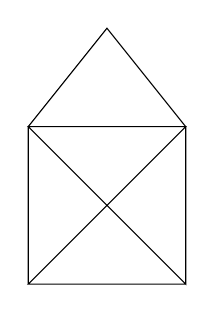
\begin{tikzpicture}
\draw (0,0) -- (0,2) -- (1,3.25) -- (2,2) -- (2,0) -- (0,2) -- (2,2) -- (0,0) -- (2,0);
\end{tikzpicture}
    
	\caption[Mit Tikz programmierte Grafik.]{Mit Tikz programmierte Grafik.}
	\label{fig:tikz_house}
\end{figure}

Ein etwas umfangreicheres Beispiel zur Digitaltechnik ist in Abbildung~\ref{fig:tikz_digital} dargestellt:

\begin{figure}[hbt]
	\centering
	\usetikzlibrary{circuits.logic.US,circuits.logic.IEC}
      \begin{tikzpicture}[circuit logic US]
      \matrix[column sep=7mm]
      {
      \node (i0) {0}; & & \\
      & \node [and gate] (a1) {}; & \\
      \node (i1) {0}; & & \node [or gate] (o) {};\\
      & \node [nand gate] (a2) {}; & \\
      \node (i2) {1}; & & \\
      };
      \draw (i0.east) -- ++(right:3mm) |- (a1.input 1);
      \draw (i1.east) -- ++(right:3mm) |- (a1.input 2);
      \draw (i1.east) -- ++(right:3mm) |- (a2.input 1);
      \draw (i2.east) -- ++(right:3mm) |- (a2.input 2);
      \draw (a1.output) -- ++(right:3mm) |- (o.input 1);
      \draw (a2.output) -- ++(right:3mm) |- (o.input 2);
      \draw (o.output) -- ++(right:3mm) node [right] {$y$ \quad Hier könnte Ihre Formel $y=(0 \land 0) \lor \overline{( 0 \land 1)}$ stehen};
 \end{tikzpicture}

	\caption[Mit Tikz programmierte Grafik, welche bereits vorgefertigte Bibliotheken für Symbole aus der Digitaltechnik nutzt.]{Mit Tikz programmierte Grafik, welche bereits vorgefertigte Bibliotheken für Symbole aus der Digitaltechnik nutzt.}
	\label{fig:tikz_digital}
\end{figure}

\clearpage

In der Tikz-Umgebung können auch Diagramme mit dem \textit{pgfplot}-Befehlssatz erzeugt werden. In Abbildung \ref{fig:pgfplot} sehen Sie ein Beispiel.

\begin{figure}[hbt]
	\centering
	\begin{tikzpicture}
		\begin{axis}[scale=1.3,legend entries={Messwerte mit Fehlerbalken,
			$\pgfmathprintnumber{\pgfplotstableregressiona} \cdot x  
			\pgfmathprintnumber[print sign]{\pgfplotstableregressionb}$}, legend style={draw=none},legend style={at={(0.01,0.98)},anchor=north west},xlabel=Stromstärke $I \; \mathrm{ \lbrack mA \rbrack}$,ylabel=Spannung $U \; \mathrm{ \lbrack V \rbrack}$]
		\addlegendimage{mark=*,blue}
		\addlegendimage{no markers,red}
\addplot+[error bars/.cd, y dir=both,y explicit]
table[x=x,y=y,y error=errory] 
{pgfplot/messdaten_mitfehler.dat};
\addplot table[mark=none,y={create col/linear regression={y=y}}]
{pgfplot/messdaten_mitfehler.dat};
	\end{axis}
\end{tikzpicture}
	\caption[Diagramm, erstellt mit dem \textit{pgfplot}-Befehlssatz.]{Ein Diagramm, erstellt in der \textit{tikzpicture}-Umgebung mit dem \textit{pgfplot}-Befehlssatz. Das Diagramm stellt Messdaten, deren Fehlerbalken und eine Regressionskurve dar. Die Messdaten werden von einer separaten Datei eingelesen und die Regressionskurve wurde mit \textit{pgfplot} berechnet und erstellt.}
	\label{fig:pgfplot}
\end{figure}

\clearpage

Auch hierzu der Quellcode in Listing~\ref{lst:pgfplot}.

\begin{lstlisting}[caption=Quellcode der Abbildung~\ref{fig:pgfplot}.,label=lst:pgfplot]
\begin{figure}[hbt]
\centering
\begin{tikzpicture}
		\begin{axis}[scale=1.3,legend entries={Messwerte mit Fehlerbalken,
			$\pgfmathprintnumber{\pgfplotstableregressiona} \cdot x  
			\pgfmathprintnumber[print sign]{\pgfplotstableregressionb}$}, legend style={draw=none},legend style={at={(0.01,0.98)},anchor=north west},xlabel=Stromstärke $I \; \mathrm{ \lbrack mA \rbrack}$,ylabel=Spannung $U \; \mathrm{ \lbrack V \rbrack}$]
		\addlegendimage{mark=*,blue}
		\addlegendimage{no markers,red}
\addplot+[error bars/.cd, y dir=both,y explicit]
table[x=x,y=y,y error=errory] 
{pgfplot/messdaten_mitfehler.dat};
\addplot table[mark=none,y={create col/linear regression={y=y}}]
{pgfplot/messdaten_mitfehler.dat};
	\end{axis}
\end{tikzpicture}
\caption[Diagramm, erstellt mit dem \textit{pgfplot}-Befehlssatz.]{Ein Diagramm, erstellt in der \textit{tikzpicture}-Umgebung mit dem \textit{pgfplot}-Befehlssatz. Das Diagramm stellt Messdaten, deren Fehlerbalken und eine Regressionskurve dar. Die Messdaten werden von einer separaten Datei eingelesen und die Regressionskurve wurde mit \textit{pgfplot} berechnet und erstellt.}
\label{fig:pgfplot}
\end{figure}
\end{lstlisting}

In Listing~\ref{lst:tikz} ist der Quellcode der Datei \textit{mess\_fehlerbalken.tex} dargestellt.

\begin{lstlisting}[caption=Quellcode der Datei \textit{mess\_fehlerbalken.tex}.,label=lst:tikz]
\begin{tikzpicture}
\begin{axis}[scale=1.3,legend entries={Messwerte mit Fehlerbalken,
$\pgfmathprintnumber{\pgfplotstableregressiona} \cdot x  
\pgfmathprintnumber[print sign]{\pgfplotstableregressionb}$}, legend style={draw=none},legend style={at={(0.01,0.98)},anchor=north west},xlabel=Stromstärke $I \; \mathrm{ \lbrack mA \rbrack}$,ylabel=Spannung $U \; \mathrm{ \lbrack V \rbrack}$]
\addlegendimage{mark=*,blue}
\addlegendimage{no markers,red}
\addplot+[error bars/.cd, y dir=both,y explicit]
table[x=x,y=y,y error=errory] 
{pgfplot/messdaten_mitfehler.dat};
\addplot table[mark=none,y={create col/linear regression={y=y}}]
{pgfplot/messdaten_mitfehler.dat};
\end{axis}
\end{tikzpicture}
\end{lstlisting}

\clearpage

In Abbildung~\ref{fig:pgfplot2y} wird ein weiters Beispiel für ein Diagramm gezeigt. Oftmals wird eine zweite y-Achse verwendet, um verschiedene Skalen darstellen zu können.

\begin{figure}[hbt]
	\centering
	\begin{tikzpicture}
%
\begin{axis}[
scale=1.3,
ytick pos=left,
xlabel=Zeit $t \; \mathrm{ \lbrack ns \rbrack}$,
ylabel=Spannung $U \; \mathrm{ \lbrack V \rbrack}$
]
\addplot[mark=*,only marks] table[x=x,y=y1] {pgfplot/messdaten_zweiyachsen.dat};
\end{axis}
%
\begin{axis}[
scale = 1.3,
legend style={draw=none},
legend style={at={(0.75,0.6)},
anchor=north west},
axis y line*=right,
axis x line=none,
%ymin=0,
%ymax=100,
ylabel=Strom $I \; \mathrm{ \lbrack mA \rbrack}$
]
\addlegendimage{mark=*,only marks}
\addlegendentry{Spannung}
\addplot[mark=x,only marks,blue] table[x=x,y=y2] {pgfplot/messdaten_zweiyachsen.dat};
\addlegendentry{Strom}
\end{axis}
\end{tikzpicture}
	\caption[Diagramm mit zwei unterschiedlichen y-Achsen.]{Diagramm mit zwei unterschiedlichen y-Achsen.}
	\label{fig:pgfplot2y}
\end{figure}

\clearpage

\subsection{Tabellen}

\begin{table}[hbt]	
	\centering
	\renewcommand{\arraystretch}{1.5}	% Skaliert die Zeilenhöhe der Tabelle
	\captionabove[Liste der verwendeten Messgeräte]{Liste der verwendeten Messgeräte. Die Genauigkeitsangaben beziehen sich auf die Standardabweichung $1\cdot \sigma$.}
	\label{tab:bsp}
	\begin{tabular}{ccccc}
		\textbf{Messgerät} & \textbf{Hersteller} & \textbf{Typ} & \textbf{Verwendung} & \textbf{Genauigkeit}\\ 
		\hline 
		\hline 
		\parbox[t]{0.2\linewidth}{\centering Spannungs-\\versorgung} & Voltmaker & HV2000 & \parbox[t]{0.2\linewidth}{\centering Spannungs-\\versorgung der\\Platine} & $\Delta U = \pm 5 $~mV \\ % Der parbox-Befehl ist erforderlich, damit ein Zeilenumbruch erzeugt werden kann. c-Spalten (zentriert) erlauben nicht automatisch einen Zeilenumpruch. Linksbündig gesetzte p-Spalten erlauben automatisch den Zeilenumbruch.
		Strommessgerät & Currentcount & Hotamp 16 & \parbox[t]{0.2\linewidth}{ \centering Strommessung\\am Versorgungspin\\des µC} & $\Delta I = \pm 0.1$~A \\ 
		\hline 
	\end{tabular} 
\end{table}

Der Quellcode der Beispieltabelle~\ref{tab:bsp} ist in Listing~\ref{lst:tab} zu sehen.

\begin{lstlisting}[caption=Quellcode der Tabelle~\ref{tab:bsp}.,label=lst:tab]
\begin{table}[hbt]	
\centering
\renewcommand{\arraystretch}{1.5}	% Skaliert die Zeilenhöhe der Tabelle
\captionabove[Liste der verwendeten Messgeräte]{Liste der verwendeten Messgeräte. Die Genauigkeitsangaben beziehen sich auf die Standardabweichung $1\cdot \sigma$.}
\label{tab:bsp}
\begin{tabular}{ccccc}
\textbf{Messgerät} & \textbf{Hersteller} & \textbf{Typ} & \textbf{Verwendung} & \textbf{Genauigkeit}\\ 
\hline 
\hline 
\parbox[t]{0.2\linewidth}{\centering Spannungs-\\versorgung} & Voltmaker & HV2000 & \parbox[t]{0.2\linewidth}{\centering Spannungs-\\versorgung der\\Platine} & $\Delta U = \pm 5 $~mV \\ % Der parbox-Befehl ist erforderlich, damit ein Zeilenumbruch erzeugt werden kann. c-Spalten (zentriert) erlauben nicht automatisch einen Zeilenumpruch. Linksbündig gesetzte p-Spalten erlauben automatisch den Zeilenumbruch.
Strommessgerät & Currentcount & Hotamp 16 & \parbox[t]{0.2\linewidth}{ \centering Strommessung\\ am Versorgungspin\\ des \textmu C} & $\Delta I = \pm 0.1$~A \\ 
\hline 
\end{tabular} 
\end{table}
\end{lstlisting}

\clearpage

\subsection{Formeln}

Formeln lassen sich in \LaTeX~ganz einfach schreiben. Es gibt unterschiedliche Umgebungen zum Schreiben von Formeln. Z.B. direkt im Text $v=s/t$ oder abgesetzt

\[F=m \cdot a\]

oder auch, wie in wissenschaftlichen Dokumenten üblich, nummeriert

\begin{equation}
P=\frac{U^2}{R} \quad .
\label{eqn:leistung}
\end{equation}

Mit einem Label in Formel~\ref{eqn:leistung} lassen sich natürlich auch Formeln im Text referenzieren. \LaTeX~verwendet im Formelmodus einen eigenen Schriftsatz, welcher entsprechend der gängigen Konventionen kursive Zeichen verwendet. Sollen im Formelmodus Einheiten in normaler Schriftart eingefügt werden, dann kann dies über den Befehl \textbackslash \textit{mathrm}\{\} erwirkt werden, wie im Quellcode von Formel~\ref{eqn:leistungMitEinh} zu sehen ist.

\begin{equation}
P=\frac{U^2}{R} = \frac{\left( 100~\mathrm{V}\right)^2}{100~\Omega} = 100~\mathrm{W}\quad .
\label{eqn:leistungMitEinh}
\end{equation}

Zum direkten Vergleich sind die Einheiten in Formel~\ref{eqn:leistungMitEinhfalsch} falsch dargestellt:

\begin{equation}
P=\frac{U^2}{R} = \frac{\left( 100~V\right)^2}{100\,\varOmega} = 100\,W
\label{eqn:leistungMitEinhfalsch}
\end{equation}

Das sind nur ein paar wenige Beispiele und es gibt sehr viele Packages, um Besonderheiten in Formeln realisieren zu können, z.B. mehrzeilige Formeln mit vertikaler Ausrichtung. Nennen Sie Formeln nur, wenn diese zum besseren Verständnis auch wirklich nützlich sind.

Folgende Befehle sind innerhalb von Formel-Umgebungen nützlich:
\begin{tabbing}
	\hspace*{0cm} \= \hspace{0.35\linewidth} \= \+\kill
	\textbackslash \textit{text}\{\}	\> Damit kann in Formel-Umgebung Text geschrieben werden.\\ 
	\textbackslash, \textbackslash: \textbackslash; oder \textbackslash quad und \textbackslash qquad \> Zusätzlichen Abstand zwischen Symbolen einfügen.\\
	\textbackslash \textit{notag} \> Nummerierung einer bestimmten Formel ausschalten.
\end{tabbing}

Abschließend nochmals ein kleines Beispiel:

\begin{eqnarray}
\sum\limits_{n=1}^\infty f\left(x_n\right)\cdot \Delta x=  \lim\limits_{\Delta x \rightarrow 0} \frac{f\left(x_0+\Delta x\right)-f\left(x_0\right)}{\Delta x} = \frac{\diff f}{\diff x} = \dot{f}(x)
\end{eqnarray}		% Zeile auskommentieren bei finalem Dokument!

\end{document}